\documentclass[a4paper,14pt]{extarticle} % класс - статья
\usepackage[utf8]{inputenc} % кодовая страница документа
\usepackage[T2A]{fontenc} % внутренняя кодировка  TeX
\usepackage[russian]{babel} % локализация и переносы

%\renewcommand{\rmdefault}{ftm}

\usepackage[top=20mm, left=30mm, right=20mm, bottom=15mm]{geometry} % поля

\usepackage{hyperref} % гиперссылки
\usepackage{cmap} % русский поиск в pdf
\usepackage{amsmath} % удобная вёрстка многострочных формул, масштабирующийся текст в формулах, формулы в рамках и др.
\usepackage{amssymb} % несколько сотен дополнительных математических символов
\usepackage{amsthm} % окружения «теорема», «лемма» и т. п.
\usepackage{amsfonts} % Ажурный \mathbb{} и готический \mathfrak{} шрифты
\usepackage{mathrsfs} % Mathematical Script letters (шрифт Эйлера) \mathscr{}
\usepackage{euscript} % Шрифт Евклида \EuScript{}
% каллиграфический шрифт \mathcal{} не требует пакета

\usepackage{setspace} % пакет для указания межстрочного интервала
\linespread{1.15} % интервал между строками
\usepackage{indentfirst} % русский стиль: отступ первого абзаца раздела
\setlength{\parskip}{0cm}
\setlength\parindent{1cm} % абзацный отступ равный по ширине 1cm

\usepackage{listings} % пакет для вставки исходного кода

\usepackage{graphicx, float} % Работа с графикой \includegraphics{}
\graphicspath{{images/referat}} % картинки в папке pictures

\usepackage[dvipsnames]{xcolor}
\newcommand{\redt}[1]{\textcolor{red}{#1}}
\newcommand{\redb}[1]{\colorbox{red}{#1}}

%\renewcommand{\theequation}{\thesection.\arabic{equation}} % двойная нумерация формул

\newcommand{\eS}{\EuScript{S}}
\newcommand{\cH}{\mathcal{H}}
\newcommand{\IN}{\subset}
\newcommand{\rr}{\mathbb{R}}
\newcommand{\0}{\varnothing}
\newcommand{\8}{\infty}

\newtheorem{theorem}{Теорема}
\newtheorem{lemma}[theorem]{Лемма}
\newtheorem{proposition}[theorem]{Предложение}
\newtheorem{corollary}[theorem]{Следствие}
\theoremstyle{definition}
\newtheorem{example}{Пример}
\newtheorem{definition}[theorem]{Определение}


\begin{document}

% Титульный лист
\thispagestyle{empty}
\begin{center}
\textbf{
Федеральное государственное учреждение науки\\
Институт математики им. С.Л. Соболева\\
Сибирского отделения Российской академии наук}
\end{center}

\noindent\rule{\textwidth}{1pt} % горизонтальная линия

\vspace{0pt plus4fill}


\begin{center}
\textbf {\large %\MakeUppercase
РЕФЕРАТ}\\
{\large Размерность самоподобных множеств, удовлетворяющих слабому условию отделимости}
\end{center}

\vspace{0pt plus4fill}

\noindent 
\hspace{8cm} Выполнил:

\hspace{8cm} аспирант ИМ СО РАН

\hspace{8cm} Дроздов Дмитрий Алексеевич


\vspace{0pt plus1fill}

\noindent 
\hspace{8cm} Научный руководитель:

\hspace{8cm} д. ф.-м. н., доцент

\hspace{8cm} Тетенов Андрей Викторович


\vspace{0pt plus4fill}
{\centering Новосибирск\ "--- 2024\par}

\newpage
\thispagestyle{empty}
\tableofcontents

\newpage
\section*{Введение}
\addcontentsline{toc}{section}{Введение}
В нашей работе мы рассматриваем самоподобные множества и их размерности подобия. 
Мы изучаем примеры, в которых размерность подобия не совпадает с размерностью Хаусдорфа.
Подходящим классом таких множеств являются самоподобные множества, копии которых пересекаются по подкопиям меньшего порядка.

Мы собираемся построить несколько примеров с перекрытиями по подкопиям и вычислить их размерность подобия.
Поскольку в таких множествах размерность Хаусдорфа будет меньше вычисленной размерности подобия, то мы представим наш пример в виде компоненты аттрактора некоторой граф-ориентированной системы, в которой копии не перекрываются друг другом.
Размерность подобия такой граф-ори\-ен\-ти\-ро\-ван\-ной системы будет совпадать с размерностью Хаусдорфа изначального множества с перекрытиями.

Построения самоподобных множеств и аттракторов граф-ори\-ен\-ти\-ро\-ван\-ных систем будут выполняться в программе {\em IFStile\/}, математические вычисления будут выполняться с помощью математического пакета {\em WolframAlpha}.

% В этом разделе показывается актуальность выбранной темы. Формулируется проблема, устанавливается цель работы, в зависимости от типа проекта могут быть сформулированы технологическое задание, задачи, и план работы над проектом. Рекомендуемый объём введения – не более 1 страницы.


\newpage
\section{Фракталы и фрактальная размерность}

\subsection{Фракталы и самоподобное множество}

Термин «фрактал» введён Бенуа Мандельбротом в 1975 году в своей фундаментальной работе <<Какова длина побережья Великобритании?>> и получил широкую известность с выходом в 1977 году его же книги «Фрактальная геометрия природы». 
Особую популярность фракталы обрели с развитием компьютерных технологий, позволивших эффектно визуализировать эти структуры. 

Поскольку фракталам присущи многие необычные свойства, многие авторы зачастую описывают их по своему. 
Здесь мы приведём определение фрактала по Фальконеру.

Когда мы называем множество $F$ фракталом, мы обычно имеем в
виду следующее:
\begin{itemize}
    \item $F$ имеет тонкую структуру, то есть обладает нетривиальной структурой на всех масштабах. В этом отличие от регулярных фигур (таких как окружность, эллипс, график гладкой функции): если рассмотреть небольшой фрагмент регулярной фигуры в очень крупном масштабе, то он будет похож на фрагмент прямой. Для фрактала увеличение масштаба не ведёт к упрощению структуры, то есть на всех масштабах можно увидеть одинаково сложную картину;
    \item $F$ слишком нерегулярно, чтобы быть описанным на традиционном геометрическом языке, как локально, так и глобально;
    \item Часто $F$ имеет некоторую форму самоподобия – они состоят из частей, которые каким-то образом напоминают целое. Иногда сходство может быть слабее, чем строгое геометрическое сходство. Так, например, сходство может быть приблизительным или статистическим;
    \item Обычно $F$ обладает дробной метрической размерностью или метрической размерностью, превосходящей топологическую. Эта размерность называется <<фрактальной размерностью>>, о ней мы ещё поговорим;
    \item Часто $F$ определяется очень простым способом, возможно, рекурсивно. Такие фракталы, несмотря на их тонкую структуру, можно визуализировать на компьютерах, используя несложный (или не очень сложный) алгоритм.
\end{itemize}

Многие объекты в природе обладают свойствами фрактала, например: побережья, облака, кроны деревьев, снежинки, система кровообращения, альвеолы и тому подобное.
Однако нас интересует один из самых простых и изученных классов фракталов --- самоподобные множества.


\begin{definition} \label{def:sss}
Пусть $\eS=\{S_1, S_2, \ldots, S_m\}$ --- это система (иньективных) сжимающих отображений евклидова пространства $\rr^n$.
Тогда существует единственное непустое компактное множество $K\IN\rr^n$, удовлетворяющее уравнению 
$$K = \bigcup \limits_{i = 1}^m S_i (K).$$ 
Такое множество $K$ называется {\em аттрактором} системы $\eS$ или {\em самоподобным} относительно $\eS$.
\end{definition}

\begin{figure}[H]
    \centering
    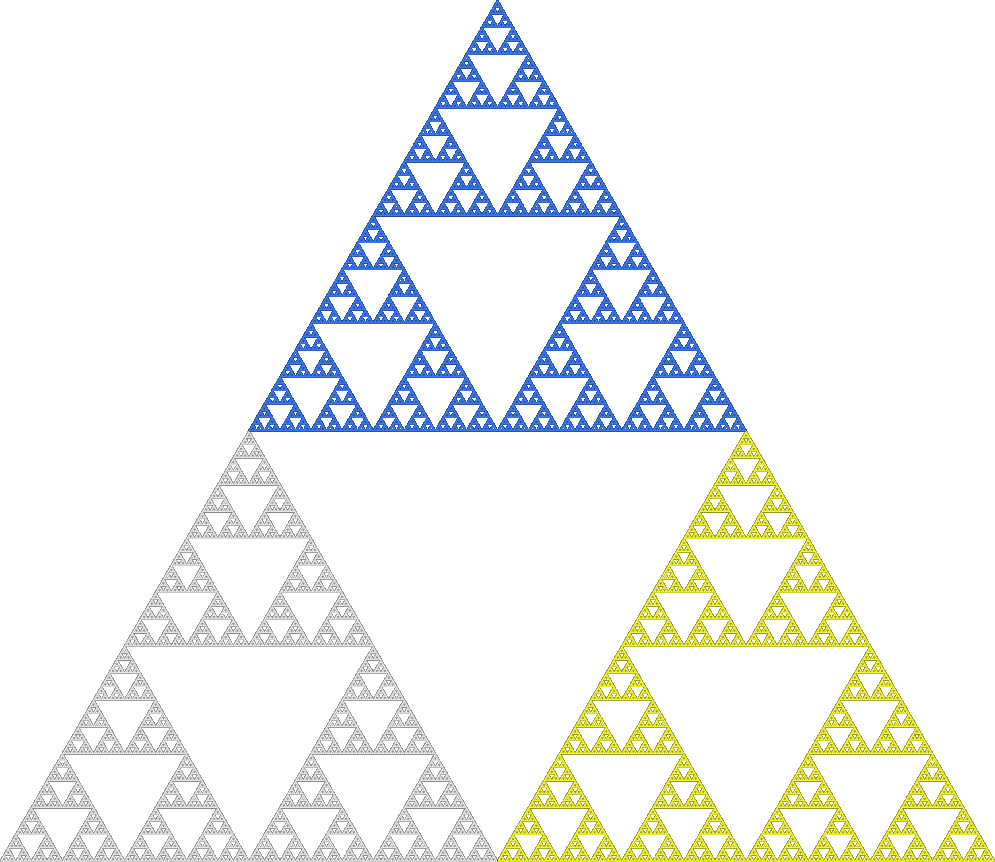
\includegraphics[width=0.45\textwidth]{Triangle_Serp.png}
    \begin{minipage}{0.85\textwidth}
        \caption{Треугольник Серпинского состоит из трёх вдвое меньших копий самого себя}
        \label{fig:serptr}
    \end{minipage}
\end{figure}

Самоподобное множество состоит из своих уменьшенных копий, но эту модель несложно обобщить.
Мы можем взять несколько множеств, состоящих как из уменьшенных копий самих себя, так и из уменьшенных копий других множеств. Такие множества называются аттрактором граф-ориентированной системы отображений. 

\begin{definition} \label{def:sss}
Пусть даны $k$ систем  $\eS_{ij}=\{S_{ij1}, S_{ij2}, \ldots, S_{ijm_{ij}}\}$ (где $i,j=1,\ldots,k$ и $m_{ij}=\#\eS_{ij}$)  сжимающих отображений евклидова пространства $\rr^n$.
Эти системы назовём граф-ориентированной системой отображений.
Тогда существует единственный набор непустых компактных множеств $K_i\IN\rr^n$, удовлетворяющих уравнениям 
$$K_i=\bigcup_{j=1}^k\eS_{ij}(K_j), \text{ где } i=1,\ldots,k.$$ 
Такие множества $K_i$ называются аттрактором граф-ориентированной системы отображений.
\end{definition}

\begin{figure}[H]
    \centering
    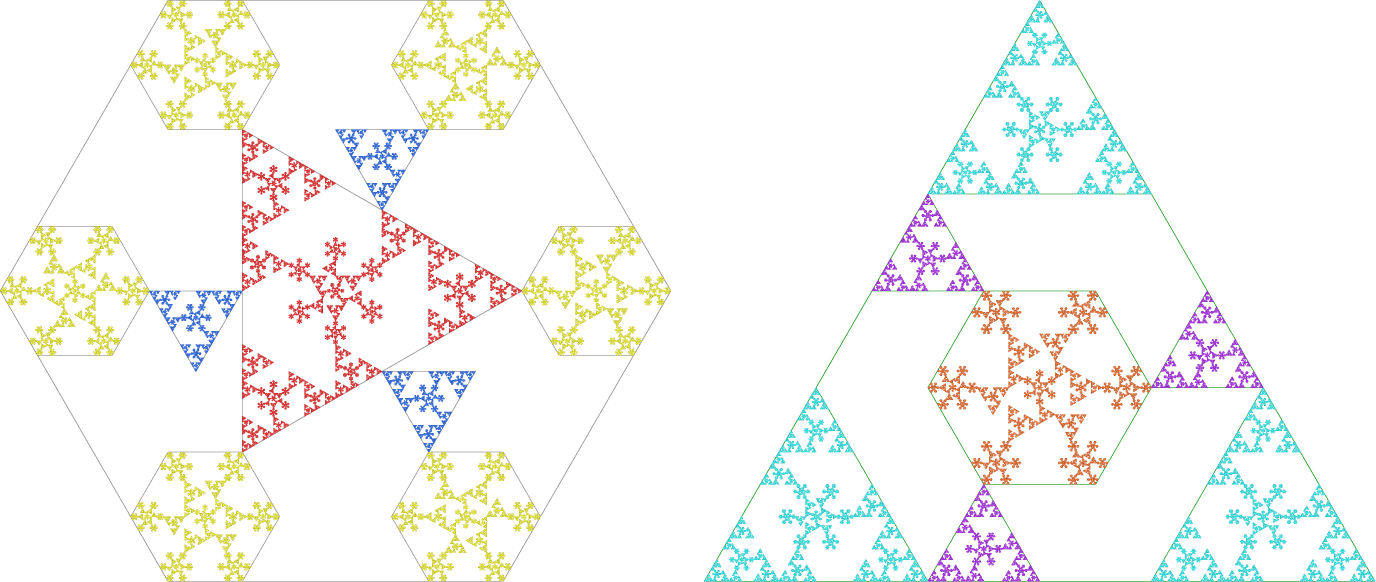
\includegraphics[width=0.8\textwidth]{gos1.png}
    \begin{minipage}{0.85\textwidth}
        \caption{Аттрактор граф-ориентированной системы из двух компонент. Каждая компонента состоит из уменьшенных копий себя и из уменьшенных копий второй компоненты.}
        \label{fig:serptr}
    \end{minipage}
\end{figure}

\subsection{Фрактальная размерность}

Понятие размерности занимает главное место во фрактальной геометрии. 
Фрактальные размерности распространяют на широкие классы множеств известное представление о том, что прямая линия или гладкая кривая одномерна, поверхность двумерна и так далее. 
Грубо говоря, размерность каким-то образом указывает, сколько места занимает множество вблизи каждой из его точек. 
Ключевым для многих определений размерности является идея "измерения множества в масштабе $\delta$". 
Для каждого $\delta$ мы измеряем множество таким образом, чтобы обнаруживать нерегулярности размера $\delta$, и мы видим, как эти измерения ведут себя при $\delta \rightarrow 0 $.

Из широкого спектра <<фрактальных размерностей>> размерность Хаусдорфа, основанная на конструкции Каратеодори, является старейшей и, вероятно, наиболее важной.
Её преимущество состоит в том, что она определяется для любого множества и основана на мерах, с которыми математически удобно работать.

Напомним, что $\delta$-покрытие множества $F$ --- это счётный (или конечный) набор множеств $\{U_i\}$ с диаметрами $0<|U_i|\leq\delta$, которые покрывают множество $F$.
Предположим, что $F$ есть подмножество в $\rr^n$, а $s\geq0$.
Для каждого $\delta>0$ мы определяем
\begin{equation}\label{eq:3_1}
    \cH_\delta^s=\inf\left\{\sum_{i=1}^\8|U_i|^s : \{U_i\} \text{ есть $\delta$-покрытие для } F\right\}.
\end{equation}
Таким образом, мы рассматриваем все покрытия множества $F$ множествами с диаметром не более чем $\delta$ и стремимся минимизировать сумму степеней $s$ диаметров.
По мере уменьшения $\delta$ класс допустимых покрытий $F$ в \eqref{eq:3_1} уменьшается.
Следовательно, инфимум $\cH_\delta^s(F)$ увеличивается или, по крайней мере, не уменьшается при $\delta\to0$ и, таким образом, приближается к пределу.
Мы запишем
\begin{equation}\label{eq:3_2}
    \cH^s(F)=\lim_{\delta\to0}\cH_\delta^s(F).
\end{equation}
Этот предел существует для любого подмножества $F$ из $\rr^n$, хотя предельное значение может быть (и обычно равно) $0$ или $\8$.
Мы называем $\cH^s(F)$ {\em $s$-мерной мерой Хаусдорфа множества $F$}.
Меры Хаусдорфа обобщают знакомые понятия длины, площади, объема и так далее.

\begin{figure}[H]
    \centering
    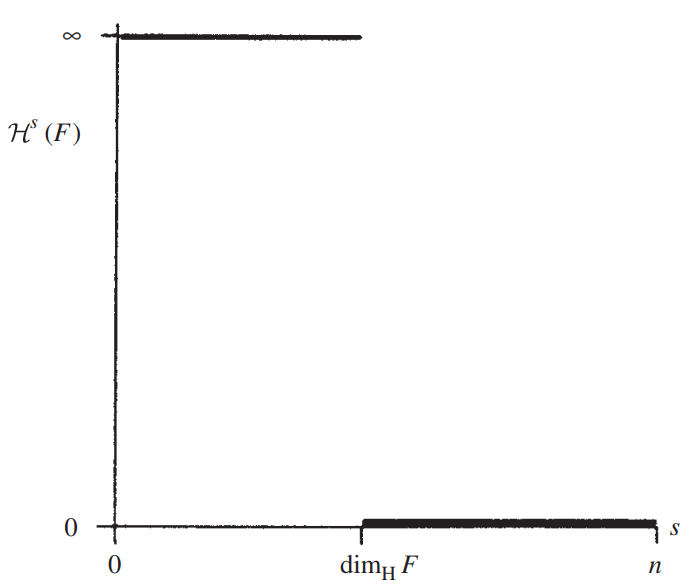
\includegraphics[width=0.4\textwidth]{dimH.png}
    \begin{minipage}{0.85\textwidth}
        \caption{}
        \label{fig:dimH}
    \end{minipage}
\end{figure}
Если мы рассмотрим график зависимости $\cH^s(F)$ от $s$ (Рис. \ref{fig:dimH}), то заметим, что существует критическое значение $s$, при котором $\cH^s(F)$ <<прыгает>> от $\8$ до $0$. 
Это критическое значение называется размерностью Хаусдорфа множества $F$, обозначается как $\dim_H(F)$. 
Оно определено для любого множества $F\IN\rr^n.$
Говоря формально (и принимая супремум пустого множества равным 0),
\begin{equation}
    \dim_H(F)=\inf\{s\geq0 : \cH^s(F)=0\}=\sup\{s :\cH^s(F)=\8\},
\end{equation}
значит 
$$\dim_H(F)=\begin{cases}
\8, & \text{ если } 0\leq s<\dim_H(F)\\
0, & \text{ если } s>\dim_H(F)
\end{cases}.$$
Если $s = \dim_H(F)$, тогда $\cH^s(F)$ может быть как нулевой или бесконечной, таи быть какой-то конечной.
%%%%%%%%%%%%%%%%%%%
Недостатком размерности Хаусдорфа является тот факт, что её зачастую трудно рассчитать или оценить с помощью вычислительных методов.
Однако для самоподобных множеств и для аттракторов граф-ориентированных систем, порождённых сжимающими подобиями, это является возможным.
Для таких множеств можно вычислить так называемую {\em размерность подобия}.

Так если копии самоподобного множества $F=\bigcup\limits_{i=1}^mS_i(F)$ пересекаются <<не слишком сильно>>, то оно имеет положительную $\cH^S$-меру.
Более того, оно удовлетворяет равенству
\begin{equation}
    \cH^s(F)=\sum_{i=1}^m \cH^s(S_i(F))=\sum_{i=1}^m r_i^s\cH^s(F),
\end{equation}
где $r_i\in(0,1)$ --- это коэффициент сжатия сжимающего подобия $S_i$.

Мы можем упростить эту формулу, условившись, что $\cH^s(F)=1$:
\begin{equation}
    \sum_{i=1}^m r_i^s=1.
\end{equation}
Вычисленная таким способом $s$ называется {\em размерностью подобия}.
Размерность подобия для граф-ориентированной системы вычисляется ненамного сложнее, примеры таких вычислений мы приведём в следующем разделе.
Так размерность подобия треугольника Серпинского на Рисунке \ref{fig:serptr} равна $\log_23$.

Размерность подобия вычисляется достаточно просто, при этом она является не только верхней границей размерности Хаусдорфа, но и почти всегда совпадает с размерностью Хаусдорфа (то есть копии самоподобного множества пересекаются <<не слишком сильно>>).

Однако в примерах самоподобных множеств, копии которых пересекаются друг с другом по подкопиям, размерность Хаусдорфа будет меньше размерности подобия.
Размерность именно таких примеров мы и рассмотрим в следующем разделе.

%%%%%%%%%%%%%%%%%%%%

% Далее рассматривается клеточная размерность, которая имеет простую интуитивно понятную формулировку и является одной из наиболее широко используемых размерностей.


% Рассматривая подмножество $F$ плоскости, для каждого $\delta>0$ мы находим наименьшее число множеств диаметром не более $\delta$, которые могут покрывать  множество $F$, и мы обозначаем это число $N_\delta (F)$, показывая число "кусочков" размера $\delta$, на которой можно разделить $F$. 
% Размерность $F$ отражает правила по которому $N_\delta (F)$ растет при $\delta \rightarrow 0 $. 
% Если $N_\delta (F)$ удовлетворяет, по крайней мере приблизительно, степенному закону $$N_\delta(F) \simeq c\delta^{-s}$$ для положительных констант $c$ и $s$ мы говорим, что $F$ имеет клеточная размерности $s$.
% Чтобы найти значение $s$, мы берем логарифмы
% \begin{equation}\label{eq:2_1}
%     \log N_\delta(F)\simeq\log c-s\log \delta,
% \end{equation}
% так    $$s \simeq \frac{\log N_\delta(F)}{-\log \delta} + \frac{\log c}{\log \delta}$$
% и мы рассчитываем получить $s$ как предел
% $$ s=\dim_{B}F=\lim_{\delta\to\ 0}\frac{\log N_\delta(F)}{-\log \delta},$$
% где второй слагаемой исчезают при переходе предел.

% Стоит отметить, что существует несколько эквивалентных определений клеточной размерности, которые иногда более удобны в использовании. Они отличаются друг от друга только определением числа $N_\delta(F)$.

% \begin{example}
% Пусть $F$ - треугольник Серпинского (рис. \ref{fig:serptr}) с длиной стороны 1. Тогда $\underline{\dim}_{B}F=\overline{\dim}_{B}F=\log 3/ \log 2$
% \end{example}

% {\it Решение.} Основное геометрическое наблюдение здесь заключается в том, что при построении, показанном на рисунке 0.3, $k$-я стадия построения состоит из $3^k$ равносторонних треугольников с длиной стороны и диаметром $2^{-k}$. Таким образом, если $2^{-k}< \delta \leq 2^{-k+1}$, $3^k$ треугольников $E_k$ дают $\delta$ покрытие $F$, поэтому $N_\delta (F)\leq 3^k$. Тогда

% $$\overline{\dim}_{B}F=\varlimsup_{\delta \to 0} \frac{\log N_\delta (F)}{-\log \delta} \leq \varlimsup_{k \to \infty} \frac{\log 3^k}{-\log 2^{-k+1}}=\frac{\log 3}{\log 2}.$$
% С другой стороны, любое множество плоскостей диаметром $\delta$, где $2^{-k-1} \leq \delta <2^{-k}$ может пересекать
% не более трех треугольников $E_k$ (такое множество не может пересекаться с парой треугольников, находящихся на расстояния больше $2^{-k}$ или друг от друга). В $E_k$,  имеется $3^k$ треугольников, каждый из которых пересекает $F$, поэтому, чтобы покрыть $F$ требуется не менее $3^k/3$ множеств диаметра меньше или равен $\delta$. Поэтому $N_\delta (F) \geq 3^{k-1}$, так что

% $$\underline{\dim}_{B}F=\varliminf_{\delta \to 0} \frac{\log N_\delta (F)}{-\log \delta} \geq \varliminf_{k \to \infty} \frac{\log 3^{k-1}}{-\log 2^{-k-1}}=\frac{\log 3}{\log 2}.$$ 


\newpage
\section{Практическая часть}

\addcontentsline{toc}{subsection}{Пример 1}
\begin{example}\label{ex:1}
Первым примером, который мы изучили, стало самоподобное множество из 5 копий (рис. \ref{fig:primer1_skelet}). 
Копии S1, S2 и S3 имеют одинаковый размер, равный $p$.
Копии S1 и S2, так же как и копии S2 и S3, пересакаются по подкопии размера $p^3$. 

\begin{figure}[H]
    \centering
    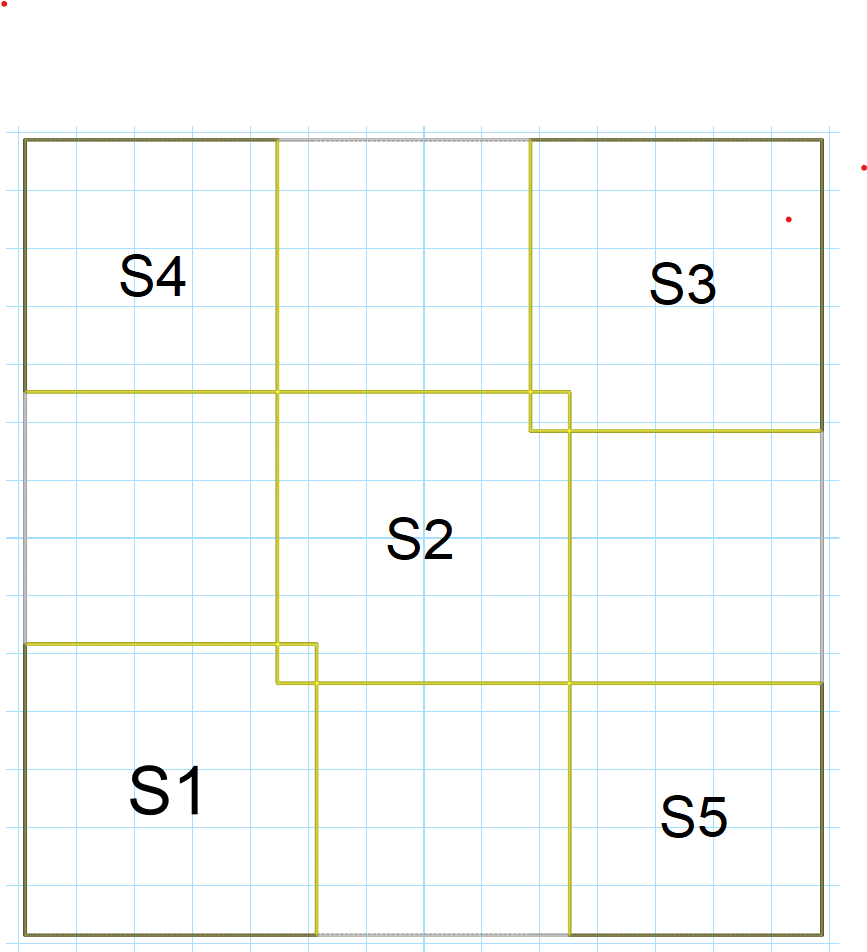
\includegraphics[width=0.48\textwidth]{3_2_скелет.png}
    \hfill
    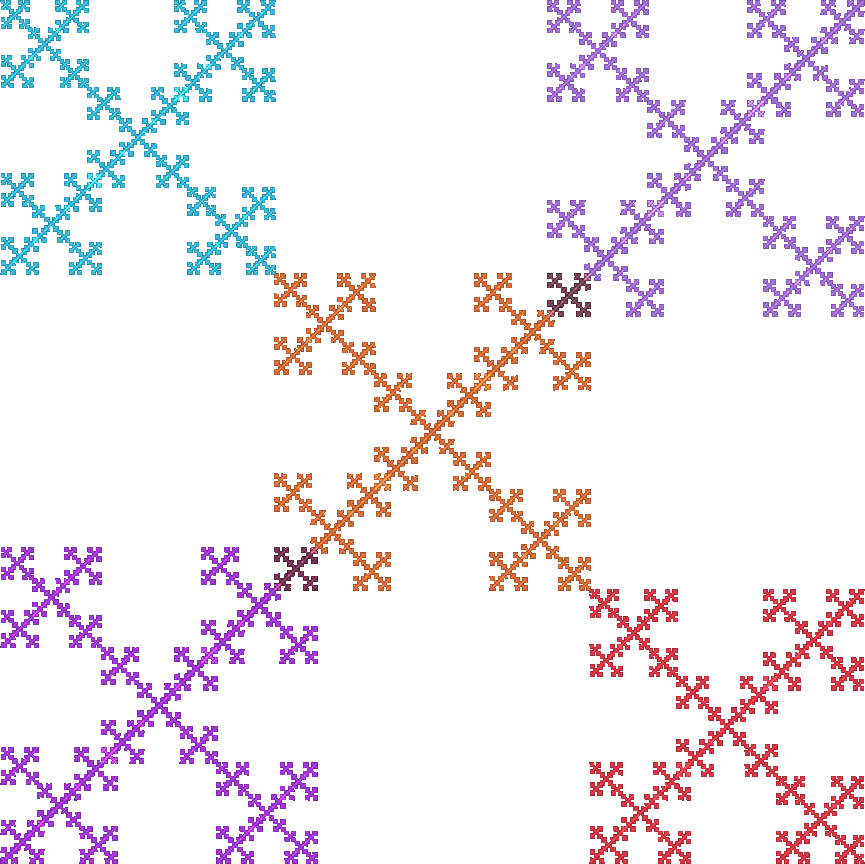
\includegraphics[width=0.45\textwidth]{3_2.png}
    \caption{Пример 1. Система из 5 копий квадрата}
    \label{fig:primer1_skelet}
\end{figure}

Значение $p$ есть корень уравнения $3p-2p^3=1$, откуда $p=\dfrac{\sqrt{3}-1}{2}$. 
Нетрудно вычислить, что размеры копий S4 и S5 равны $q=\dfrac{3-\sqrt{3}}{4}$.

Вычислим размерность подобия аттрактора (Рисунок \ref{fig:primer1_skelet} справа):
$$3p^s+2q^s=1,\;\text{ откуда }\; s\approx1.5199486042.$$


% В данном примере дважды встречается пересечение копий по подкопии третьего порядка, в связи с чем размерность подобия не совпадает с размерностью Хаусдорфа. 
% Чтобы вычислить настоящую размерность фрактала, мы представили его как граф-ориентированную систему, состоящую из двух аттракторов, в которой нет пересечений по подкопиям (рис. \ref{fig:primer1_1_2}).

Поскольку в аттракторе встречаются перекрытия копий по подкопиям, то при таком вычислении размерности меры этих подкопий учитываются несколько раз. 
Значит размерность Хаусдорфа этого множества будет меньше, чем вычисленная размерность подобия. 

\begin{figure}[H]
    \centering
    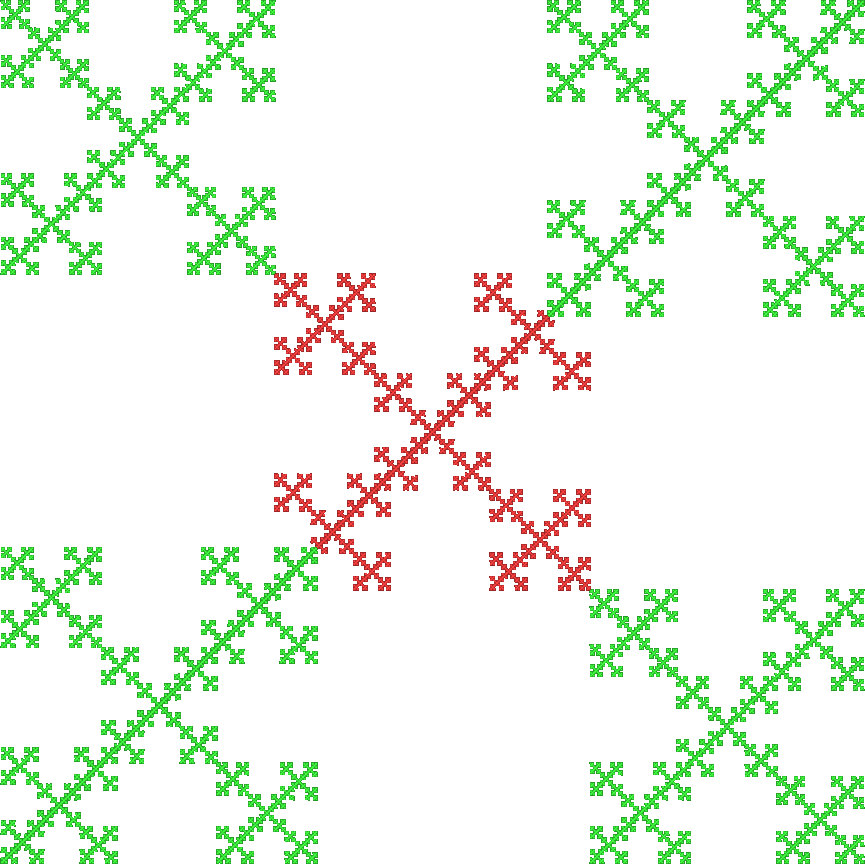
\includegraphics[width=0.45\textwidth]{3_2_1.png}
    \hfill
    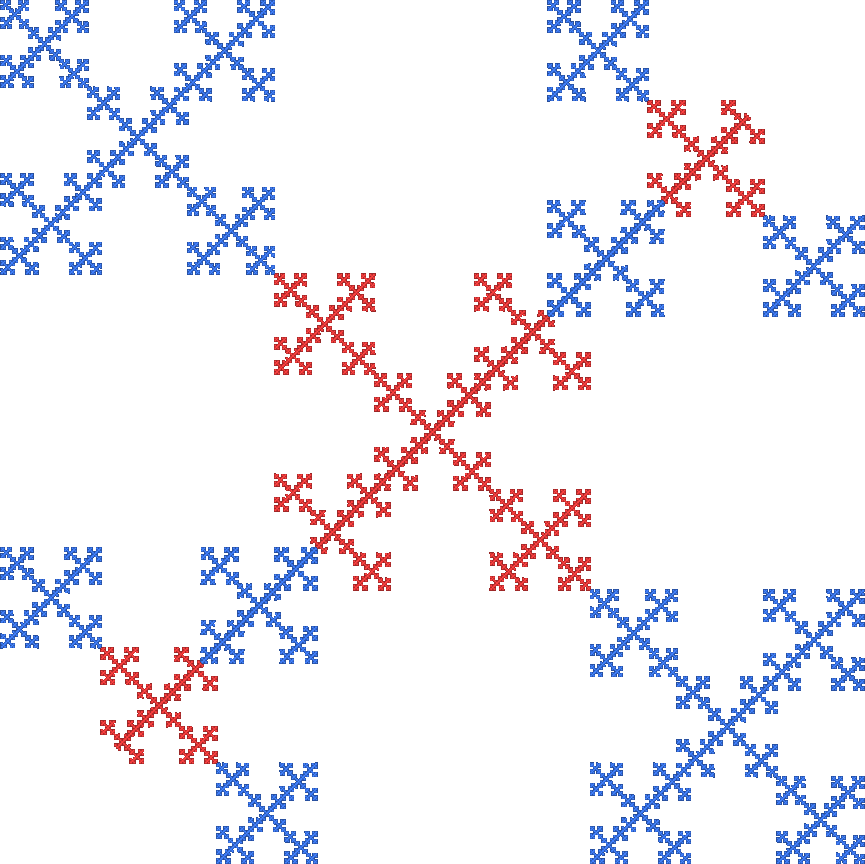
\includegraphics[width=0.45\textwidth]{3_2_2.png}
    \begin{minipage}{0.85\textwidth}
        \caption{Аттрактор граф-ориентированной системы для примера \ref{ex:1}. Зелёные и синие части являются копиями левого множества, а красные являются копиями правого множества}
        \label{fig:primer1_1_2}
    \end{minipage}
\end{figure}


Для вычисления этой размерности Хаусдорфа можно представить это самоподбное множество как компоненту аттрактора граф-ори\-ен\-ти\-ро\-ван\-ной системы без перекрытий. 
Пример такого аттрактора показан на Рисунке \ref{fig:primer1_1_2}, а размерность подобия этой граф-ори\-ен\-ти\-ро\-ван\-ной системы будет равна нужной нам размерности Хаусдорфа.
В отличии от размерности подобия обычного самоподобного множества, размерность подобия аттрактора граф-ори\-ен\-ти\-ро\-ван\-ной системы выражается в системе уравнений.
Запишем, при $p=\dfrac{\sqrt{3}-1}{2}$ и $q=\dfrac{3-\sqrt{3}}{4}$, эту систему:
$$
\begin{cases}
(2+a)p^s+2q^s=1\\
6p^{2s}+ap^s+2a(pq)^s+2q^s=a
\end{cases}
$$

Отсюда находим размерность подобия $s\approx1.4995614213$ этой граф-ориентированной системы, которая совпадает с размерностью Хаусдорфа искомого фрактала с перекрытием. 
\end{example}


\addcontentsline{toc}{subsection}{Пример 2}
\begin{example}\label{ex:2}
Следующим примером в нашем исследовании стало самоподобное множество, состоящее из 5 копий. (рис. \ref{fig:primer2_skelet}) 
Копии S1, S2, S3, S4 имеют одинаковый размер, копия S5 пересекается с копиями S1, S2, S3 и S4 по подкопии третьего порядка. 

\begin{figure}[H]
    \centering
    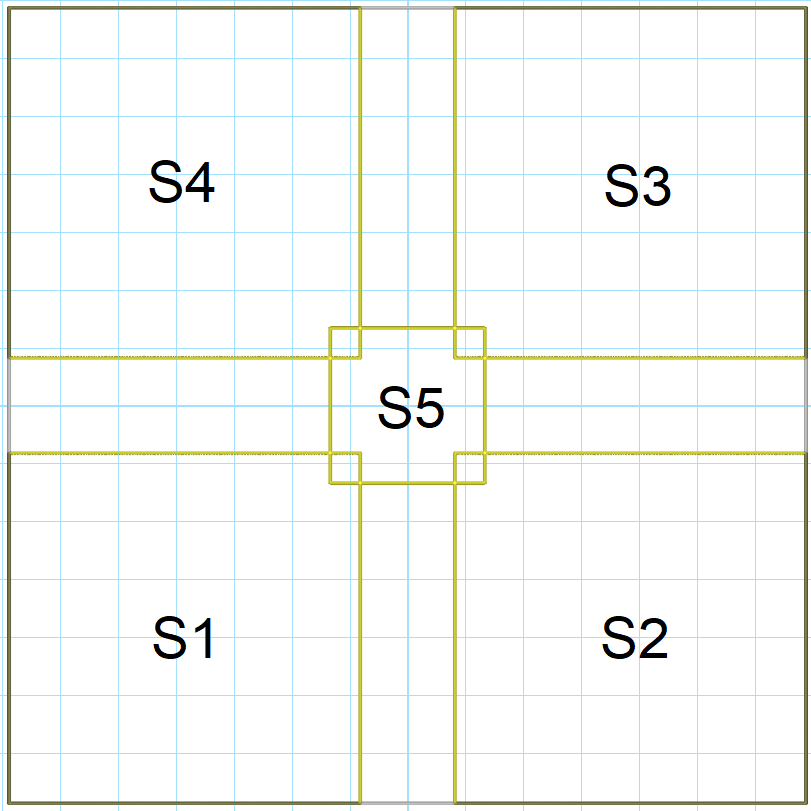
\includegraphics[width=0.45\textwidth]{1_1_скелет.png}
    \hfill
    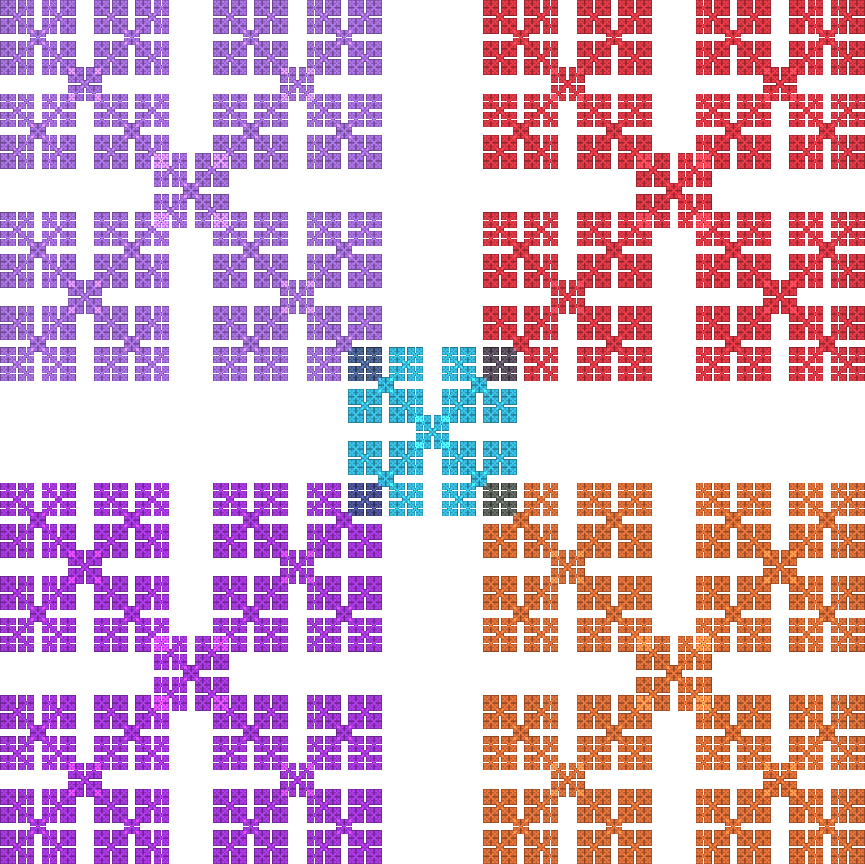
\includegraphics[width=0.45\textwidth]{1_1.png}
    \caption{Пример 2}
    \label{fig:primer2_skelet}
\end{figure}
В данном примере четыре раза встречается пересечение копий по подкопиям третьего порядка, поэтому размерность подобия отличается от размерности Хаусдорфа. 
Вычислим размер копий. Пусть длина стороны исходного квадрата равна 1, и пусть размер угловых копий  равен $p$, а размер копии в центре равен $q$.
Тогда справедлива система уравнений:
$$
\begin{cases}
p^4 = p^2q\\
2p + q - 2p^4 = 1
\end{cases}
$$
Откуда имеем $p\approx0.4406197005$ и $q=p^2\approx0.1941457205$.
При заданных $p$ и $q$ вычислим размерность подобия $s$ этого аттрактора:\\
$4p^s+q^s=1$, а значит $s\approx1.7614480242$. 

В данном аттракторе встречаются перекрытия копий по подкопиям и поэтому при подсчете размерности подобия эти участки учитываются многократно, поэтому эта размерность не является настоящей. 

Вновь для вычисления настоящей размерности исследуемого фрактала представим его как компоненту аттрактора граф-ориентированной системы без перекрытий (см. Рисунок \ref{fig:primer2}).
Пусть $a$ -- мера второго аттрактора граф-ориентированной системы, $1$ -- мера первого, тогда имеет место система:
$$
\begin{cases}
   4p^s + aq^s = 1\\
   12p^{2s} + 4a(pq)^{s} +aq^s  = a
\end{cases}
$$
В итоге имеем $s\approx1.7454704511$. Это и есть размерность граф-ори\-ен\-ти\-ро\-ван\-ной системы, она совпадает с размерностью Хаусдорфа изначального фрактала с перекрытием.

\begin{figure}[H]
    \centering
    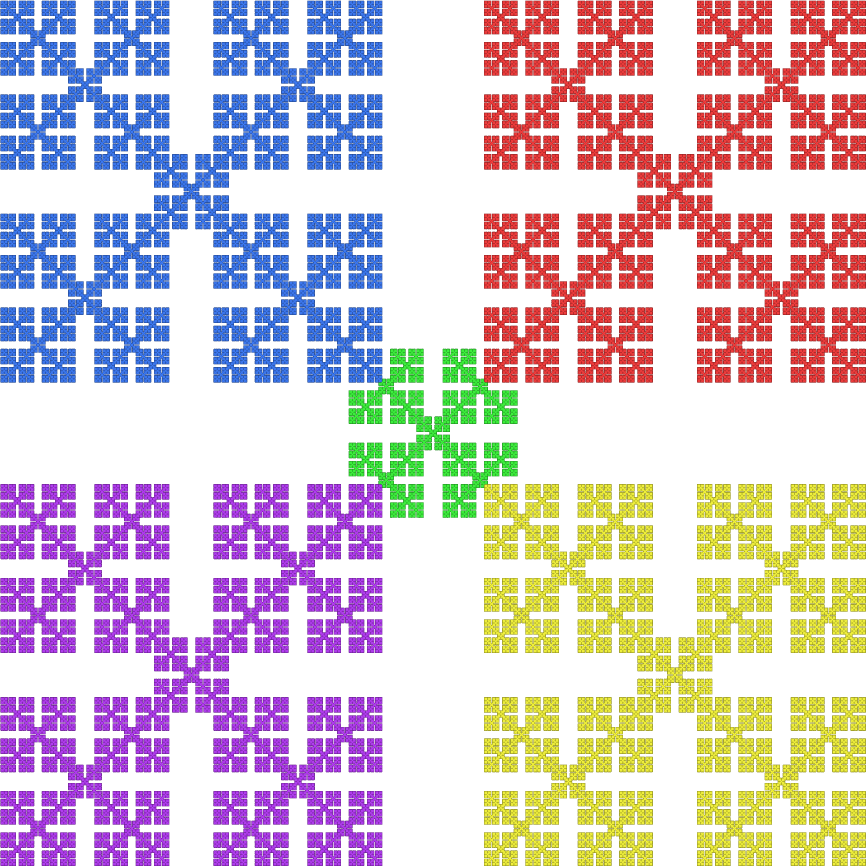
\includegraphics[width=0.45\textwidth]{1_1_1.png}
    \hfill
    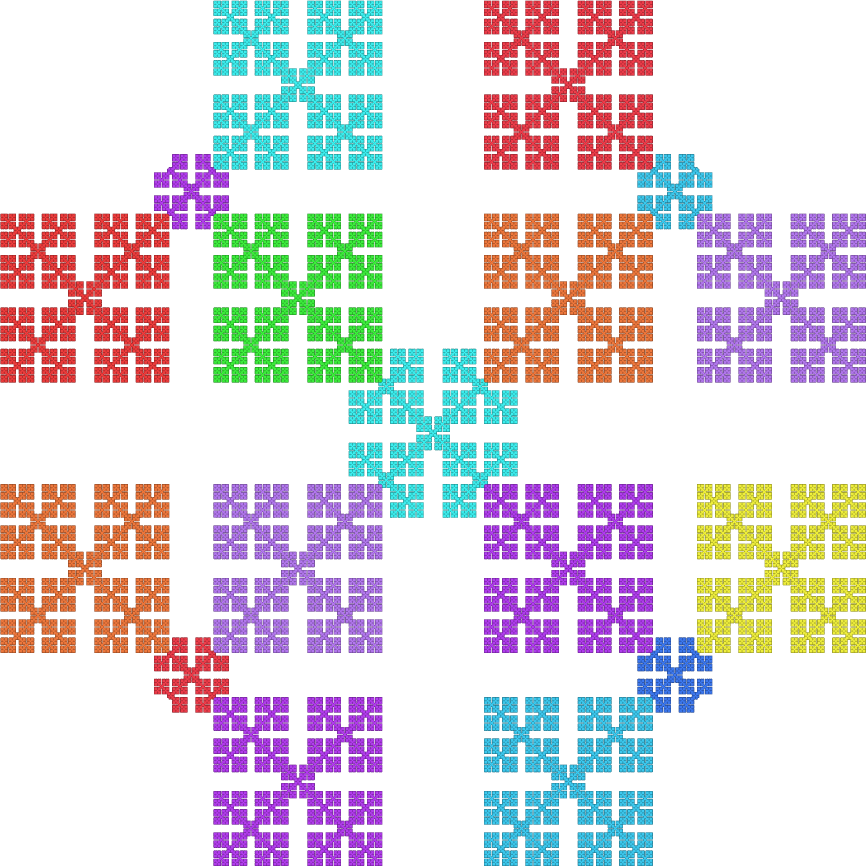
\includegraphics[width=0.45\textwidth]{1_1_2.png}
    \caption{Аттрактор граф-ориентированной системы примера \ref{ex:2}}
    \label{fig:primer2}
\end{figure}
\end{example}


\addcontentsline{toc}{subsection}{Пример 3}
\begin{example}\label{ex:3}
Третьим примером в нашем исследовании стало самоподобное множество, состоящее из семи копий треугольника. (рис. \ref{fig:pr3_скелет})
Размер копий S1, S2, S3 равен $p\approx0.3949308436$, копий S5, S6, S7 равен $p^2$, а копия S7 имеет размер $q\approx0.3072307741$.
В примере трижды встречается пересечение по подкопии размера $p$.

\begin{figure}[H]
    \centering
    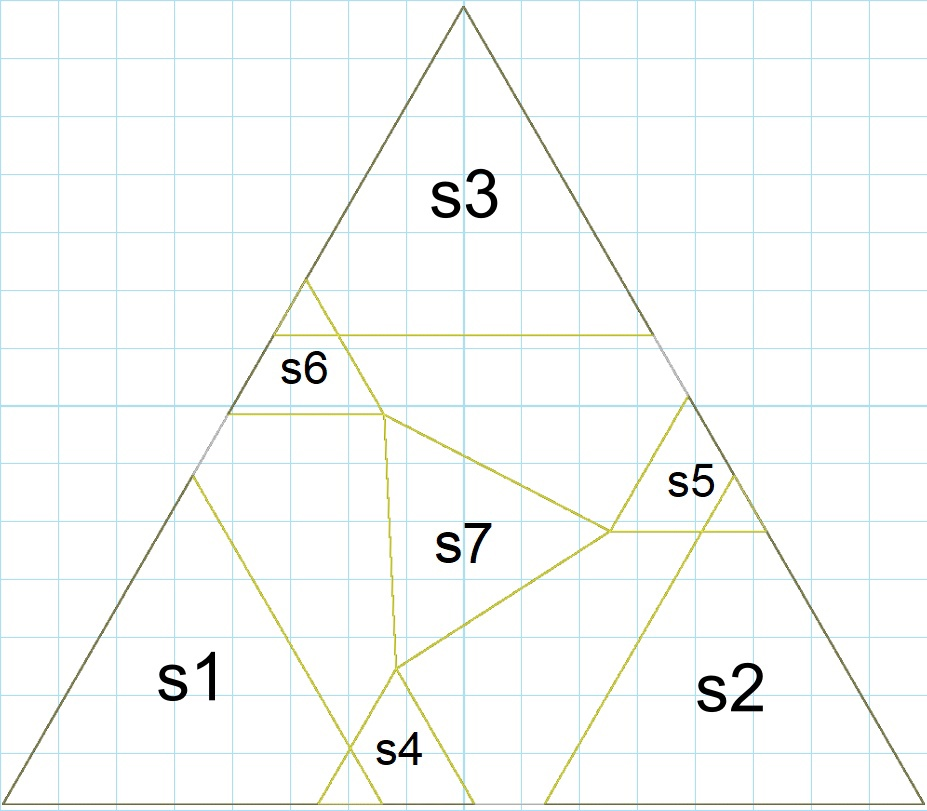
\includegraphics[width=0.45\textwidth]{den_tr_скелет.png}
    \hfill
    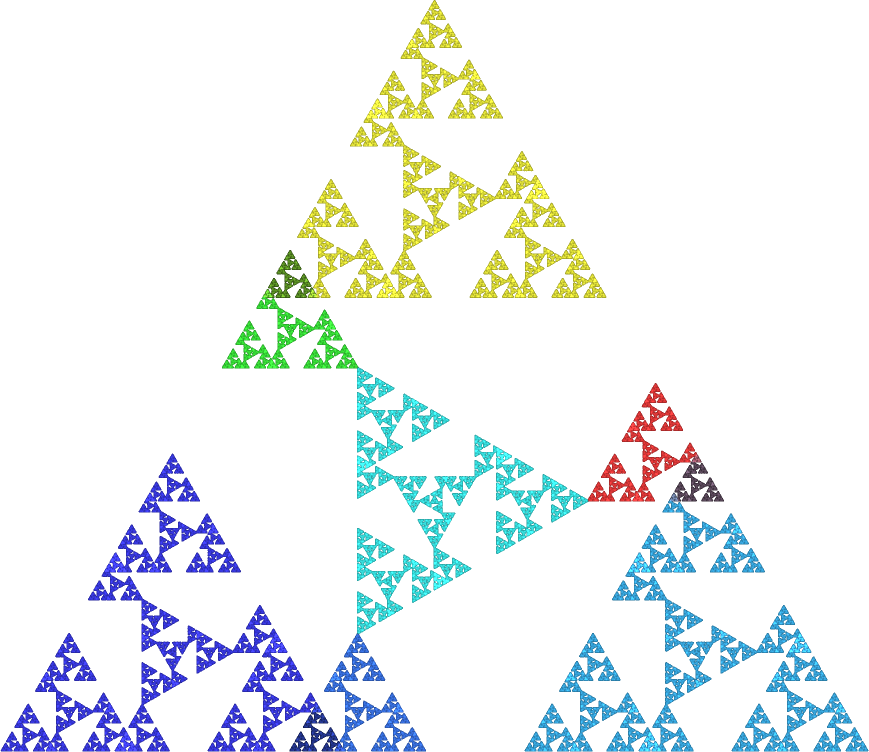
\includegraphics[width=0.45\textwidth]{den_tr.png}
    \caption{Пример 3}
    \label{fig:pr3_скелет}
\end{figure}
Размерность подобия такого множества есть $s\approx1.5848570299$, так как
$$3p^s + 3p^{2s} + q^s = 1.$$

\begin{figure}[H]
    \centering
    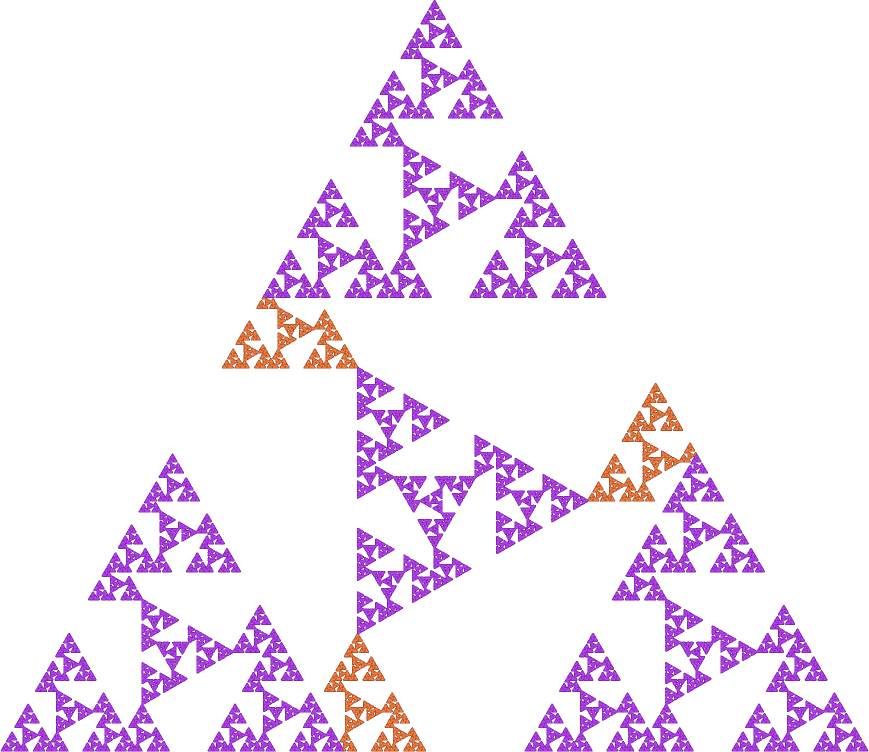
\includegraphics[width=0.45\textwidth]{den_tr_1.png}
    \hfill
    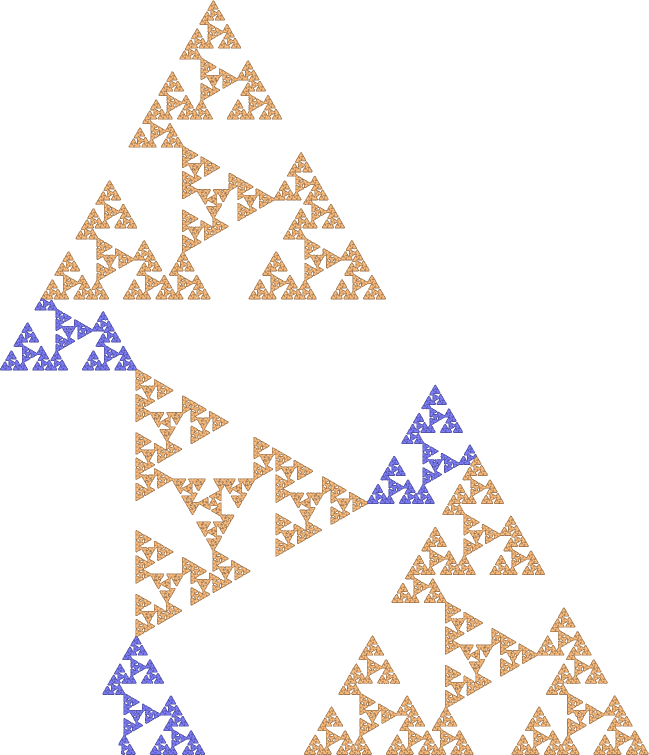
\includegraphics[width=0.32\textwidth]{den_tr_2.png}
    \caption{Аттрактор граф-ориентированной системы для примера \ref{ex:3}}
    \label{fig:pr3}
\end{figure}

Для вычисления размерности Хаусдорфа этого множества мы построили граф-ориентированную систему без перекрытий (см. Рисунок \ref{fig:pr3}) и нашли её размерность подобия:
$$
\begin{cases}
3p^s + q^s + 3ap^{2s} = 1\\
2p^s + q^s + 3ap^{2s} = a
\end{cases}
$$
Значит размерность Хаусдорфа есть $s\approx1.5487824822$.
\end{example}


\addcontentsline{toc}{subsection}{Пример 4}
\begin{example}\label{ex:4}
Рассмотрим множество, состоящее из четырёх копий размера $1/2$.
Первая и четвёртая копии пересекаются со второй копией по подкопиям второго порядка размера $1/4$.
\begin{figure}[H]
    \centering
    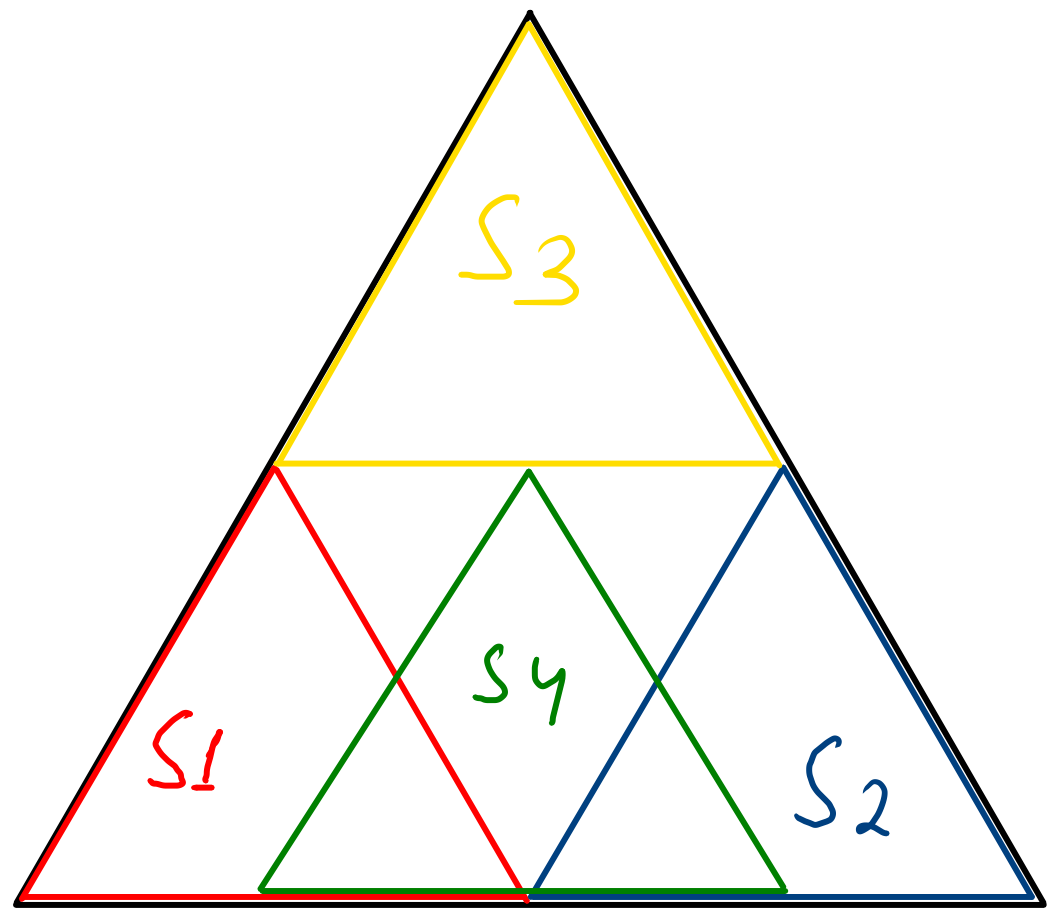
\includegraphics[width=0.45\textwidth]{e4k1.png}
    \hfill
    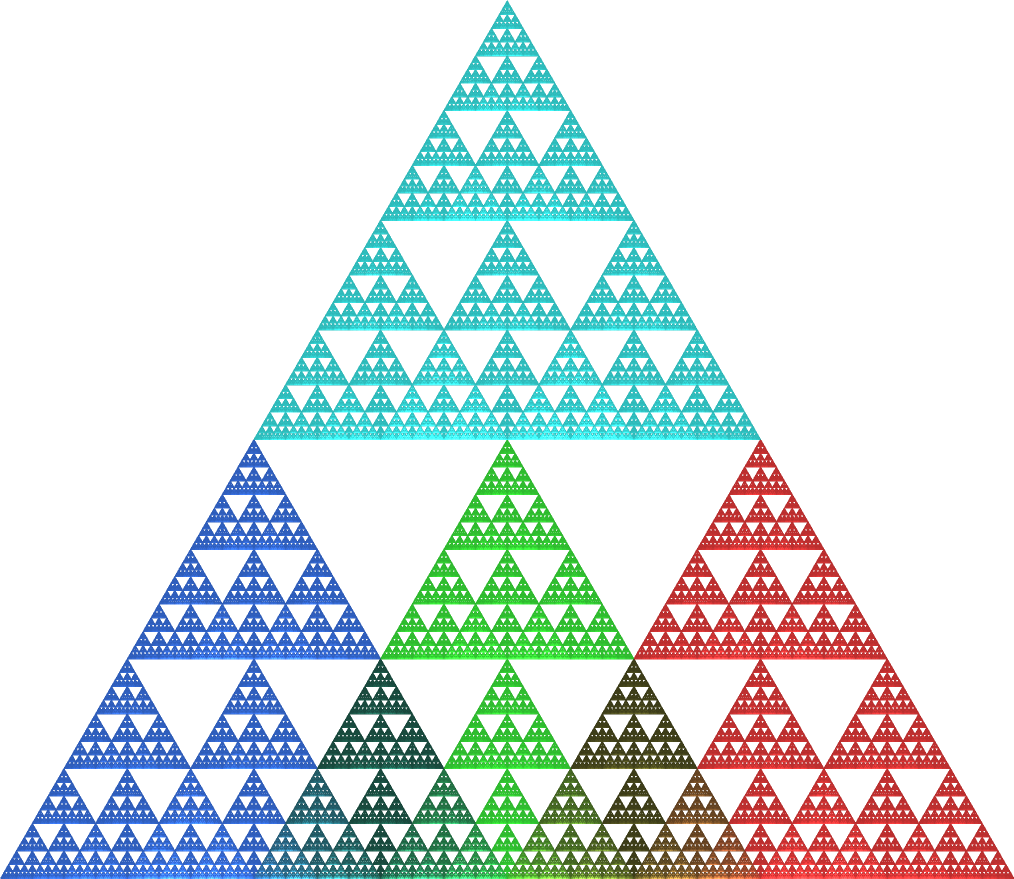
\includegraphics[width=0.45\textwidth]{e4k.png}
    \begin{minipage}{0.85\textwidth}
        \caption{Пример 4}
        \label{fig:ex4}   
    \end{minipage}
\end{figure}

Размерность подобия такого фрактала легко вычисляется по формуле:
$$4\cdot0.5^s=1\;\text{ а значит }\;s=\log_24=2$$

%Из-за перекрытий размерность Хаусдорфа будет меньше, чем такая размерность подобия.
Этот пример мы представили как компоненту граф-ориентированной системы без перекрытий, примем двумя разными способами (см Рисунки \ref{fig:ex4gds1} и \ref{fig:ex4gds2}).

Вычислим размерности подобия этих граф-ориентированных систем.

\begin{figure}[H]
    \centering
    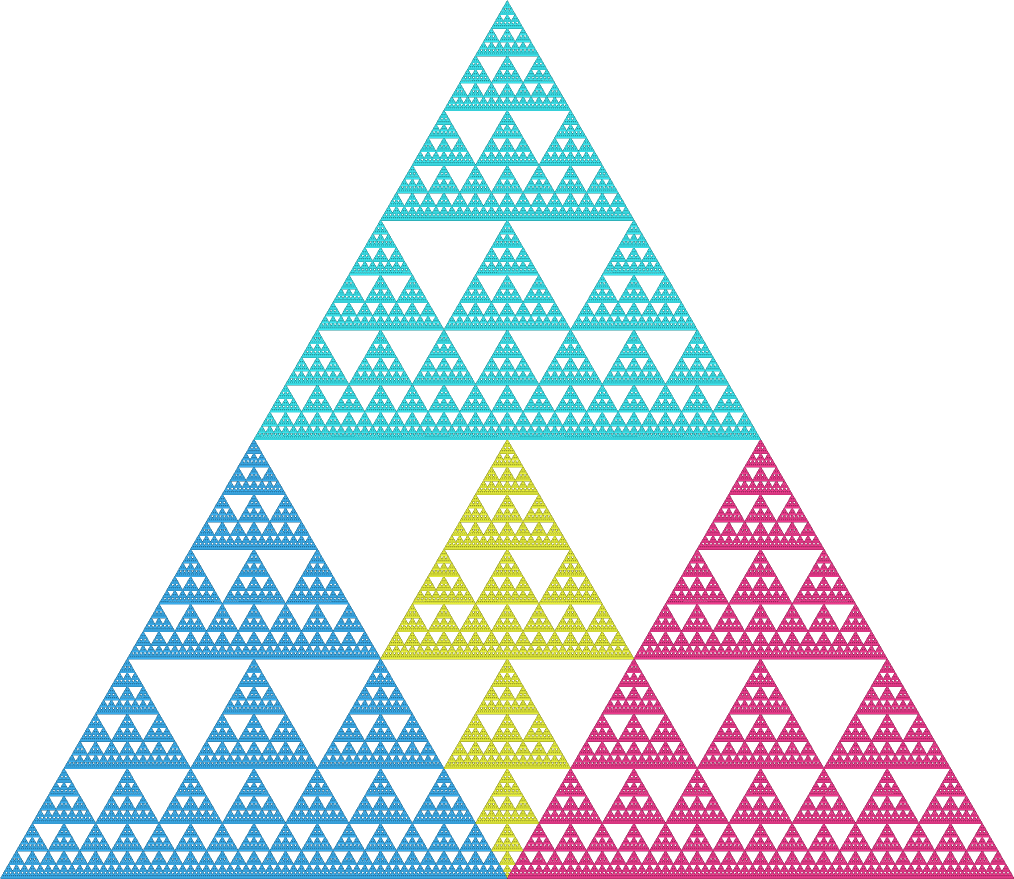
\includegraphics[width=0.5\textwidth]{e4a.png}
    \hfill
    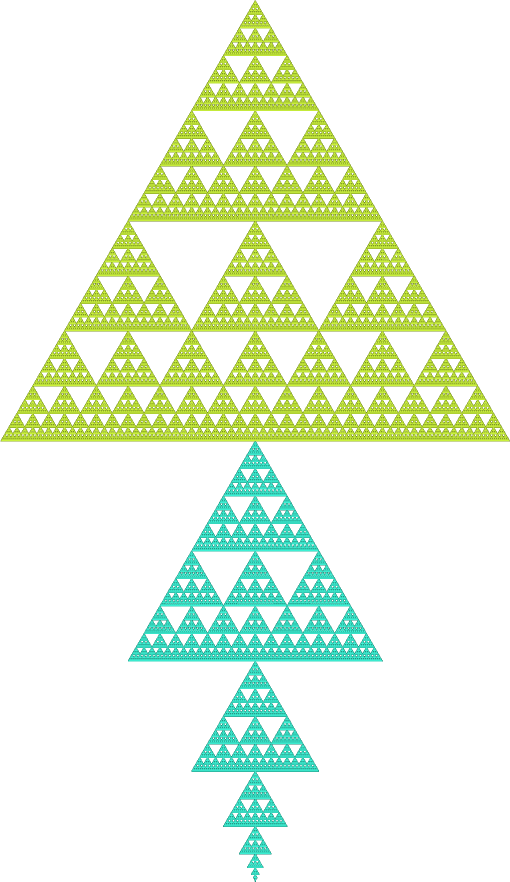
\includegraphics[width=0.25\textwidth]{e4b.png}
    \begin{minipage}{0.85\textwidth}
        \caption{Аттрактор граф-ориентированной системы для примера \ref{ex:4} (Вариант 1)}
        \label{fig:ex4gds1}   
    \end{minipage}
\end{figure}
$$
\begin{cases}
   3\cdot0.5^s + a\cdot0.5^s = 1\\
   0.5^s + a\cdot0.5^s= a
\end{cases}
\;\text{ а значит }\;s=\log_{2}(2+\sqrt2)\approx1.771553
$$


\begin{figure}[H]
    \centering
    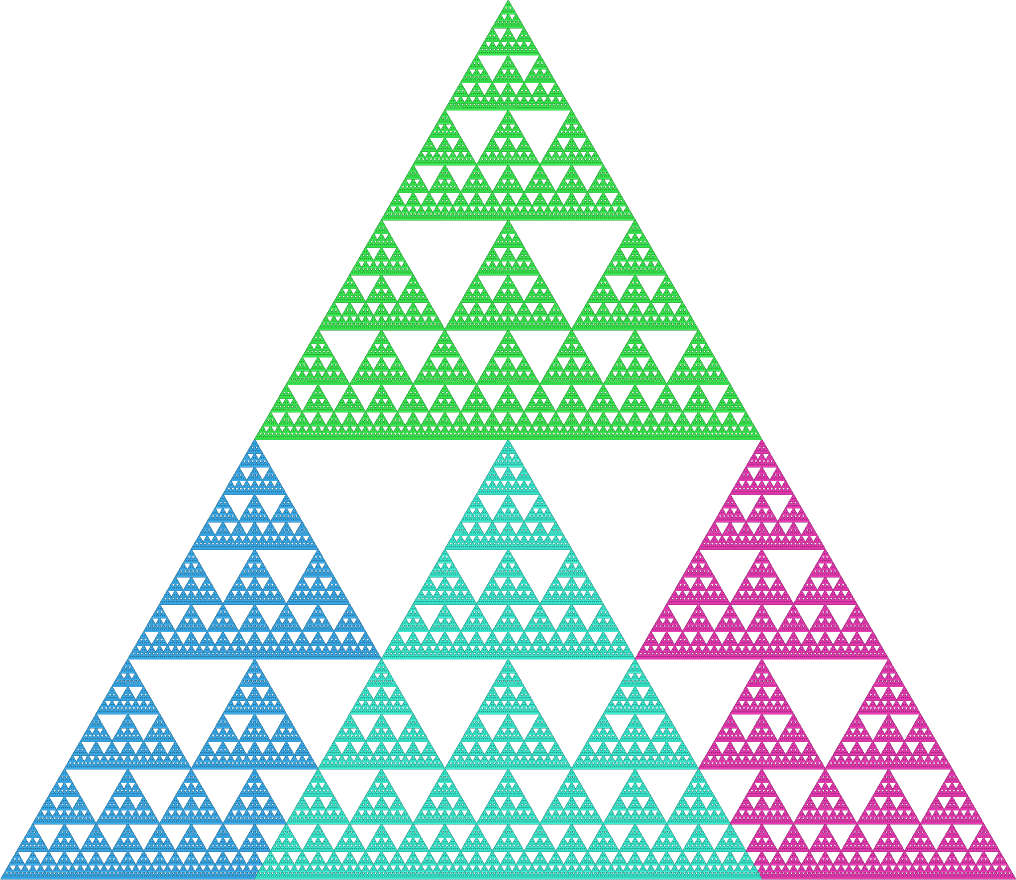
\includegraphics[width=0.3\textwidth]{e4x.png}
    \hfill
    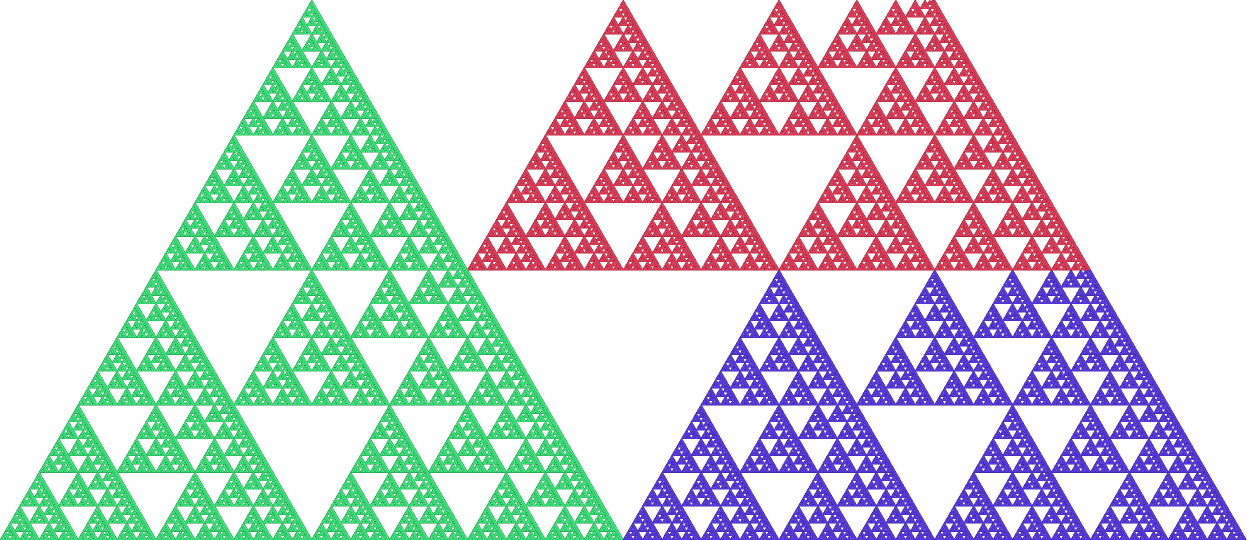
\includegraphics[width=0.3\textwidth]{e4y.png}
    \hfill
    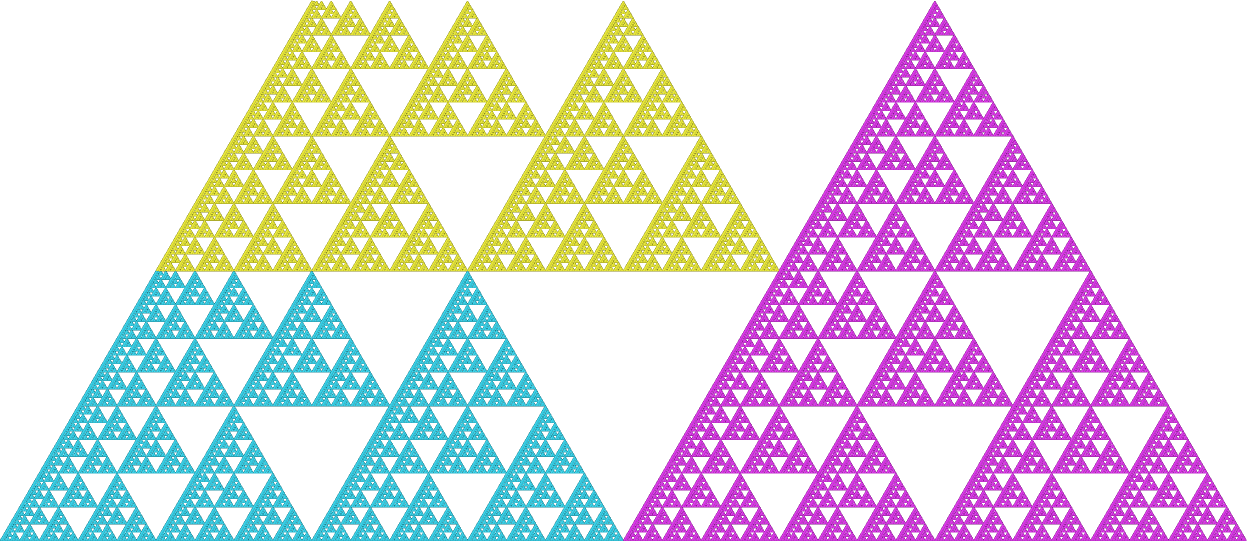
\includegraphics[width=0.3\textwidth]{e4z.png}
    \begin{minipage}{0.85\textwidth}
        \caption{Аттрактор граф-ориентированной системы для примера \ref{ex:4} (Вариант 2)}
        \label{fig:ex4gds2}   
    \end{minipage}
\end{figure}

$$
\begin{cases}
   2\cdot0.5^s + 2a\cdot0.5^s = 1\\
   0.5^s + 2a\cdot0.5^s= a
\end{cases}
\;\text{ а значит }\;s=\log_{2}(2+\sqrt2)\approx1.771553
$$
Этим мы демонстрируем тот факт, что пример с перекрытием можно представить как компоненту аттрактора ГОС без перекрытий разными способами, причём размерности подобия этих систем будут совпадать.
\end{example}


\addcontentsline{toc}{subsection}{Пример 5}
\begin{example}\label{ex:5}

Последним и самым сложным примером для изучения стала система из 13 копий (рис. \ref{fig:primer5_скелет}).
В системе 6 копий имеют размер $a$, 6 копий имеют размер $a^2$, есть одна копия (в центре) размера $1-2a-2a^2+2a^4$.
В системе есть 6 перекрытий по подкопиям размера $a^3$ и 3 перекрытия по подкопиям размера $a^4$.
Число $a$ есть корень уравнения $4a-3a^3=1$, откуда $a=\dfrac{\sqrt{5}-1}{4}$.

\begin{figure}[H]
    \centering    
    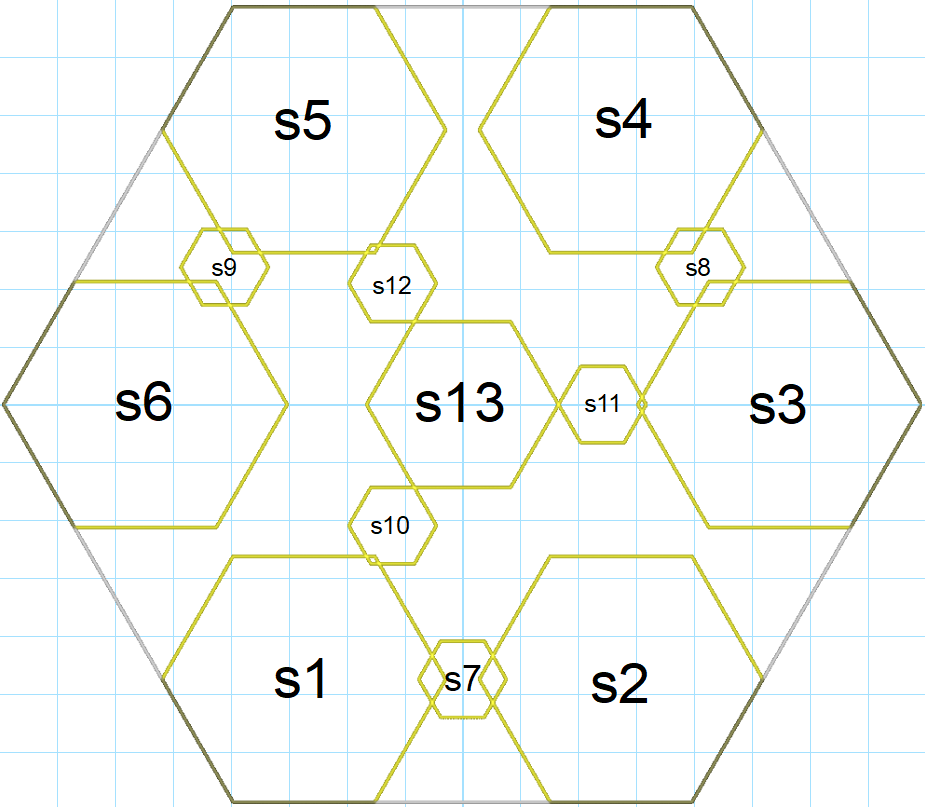
\includegraphics[width=0.45\textwidth]{extreme_skel_pod.png}
    \hfill
    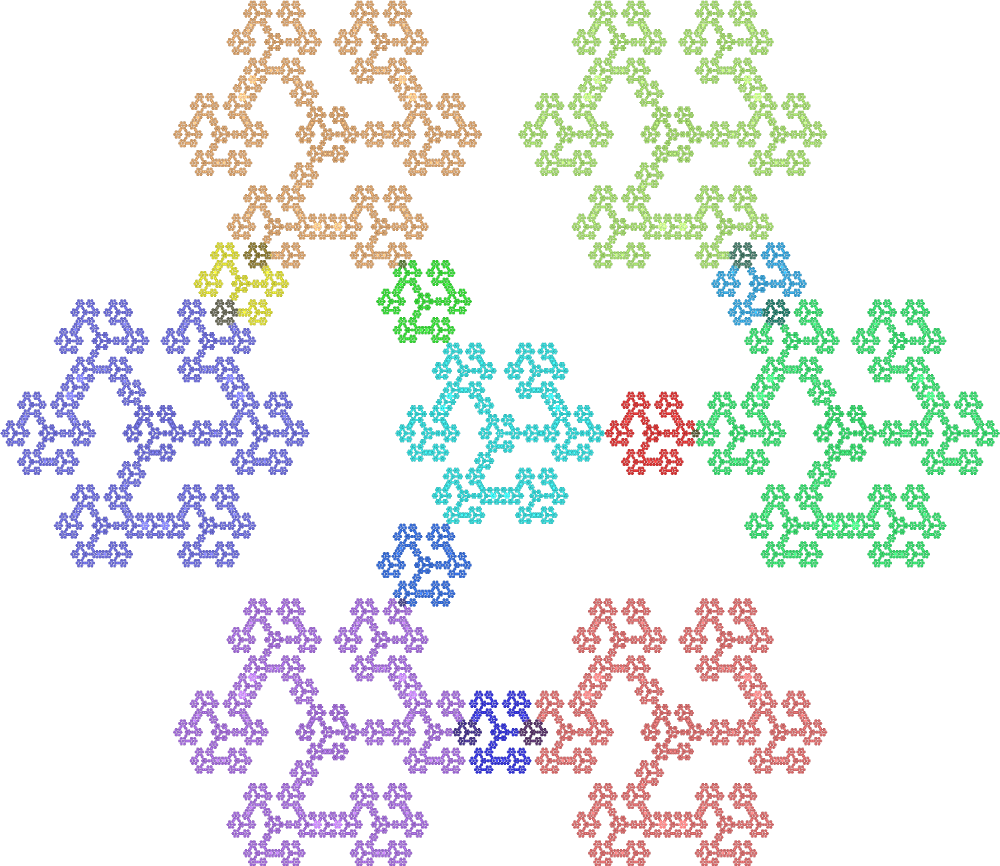
\includegraphics[width=0.45\textwidth]{den_six_3_2_4_3_full.png}
    \caption{Пример 5. Шестиугольник}
    \label{fig:primer5_скелет}
\end{figure}
Мы вычислили размерность подобия $s$ этого аттрактора:
$$6a^s+6a^{2s}+(1-2a-2a^2+2a^4)^s=1,\;\text{ откуда }\; s\approx1.69669525348048.$$

\begin{figure}[H]
    \centering
    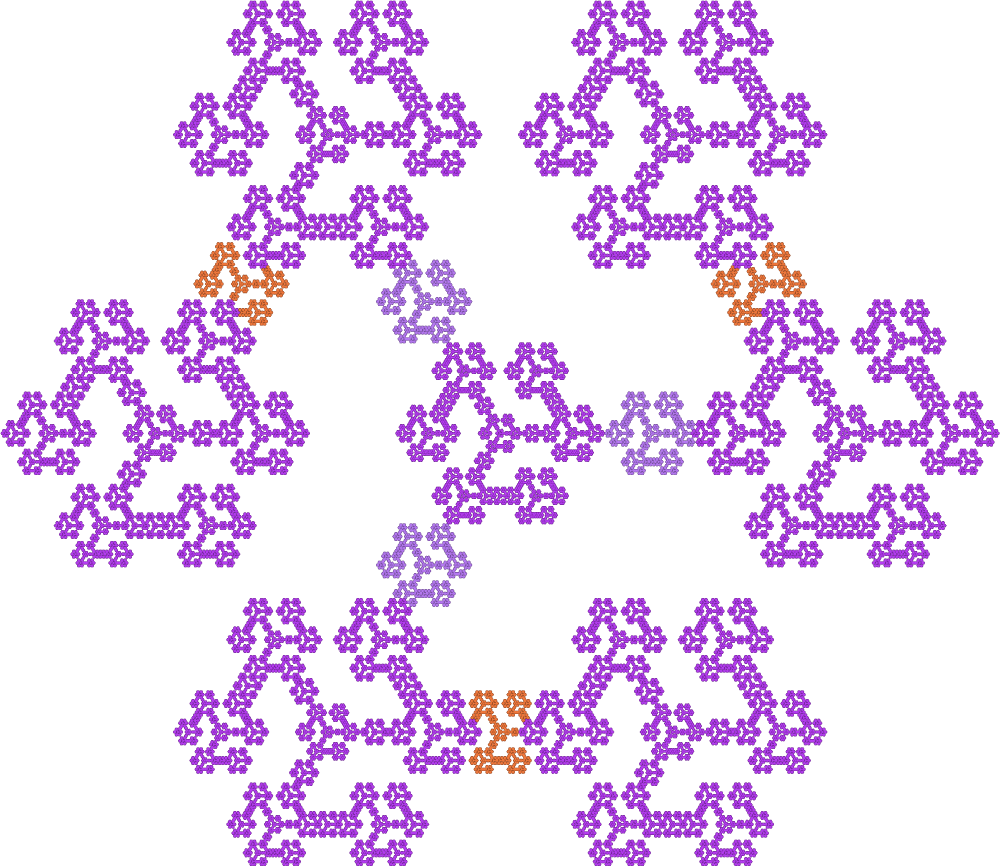
\includegraphics[width=0.35\textwidth]{EXTREME_5.1.png}
    \hfill
    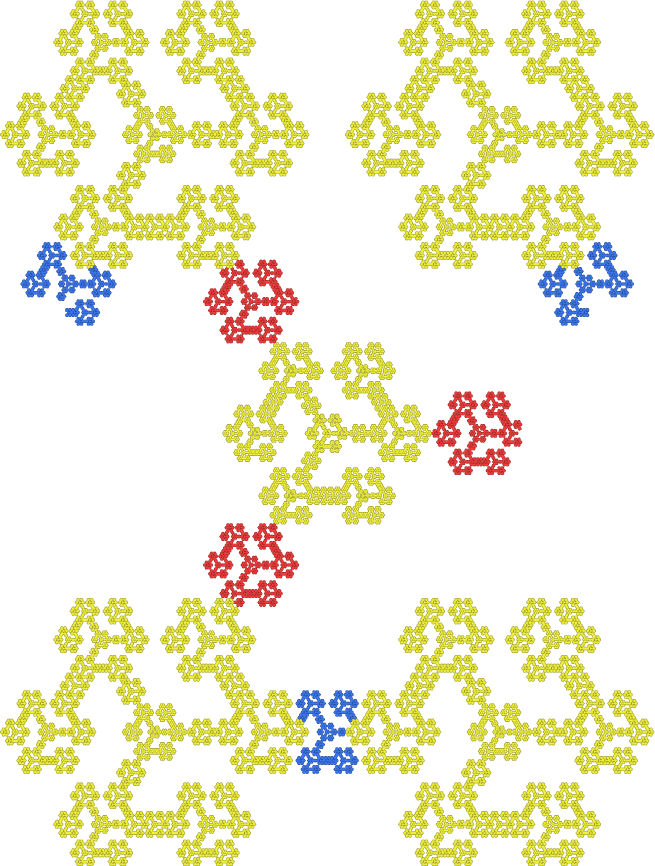
\includegraphics[width=0.23\textwidth]{EXTREME_5.2.png}
    \hfill
    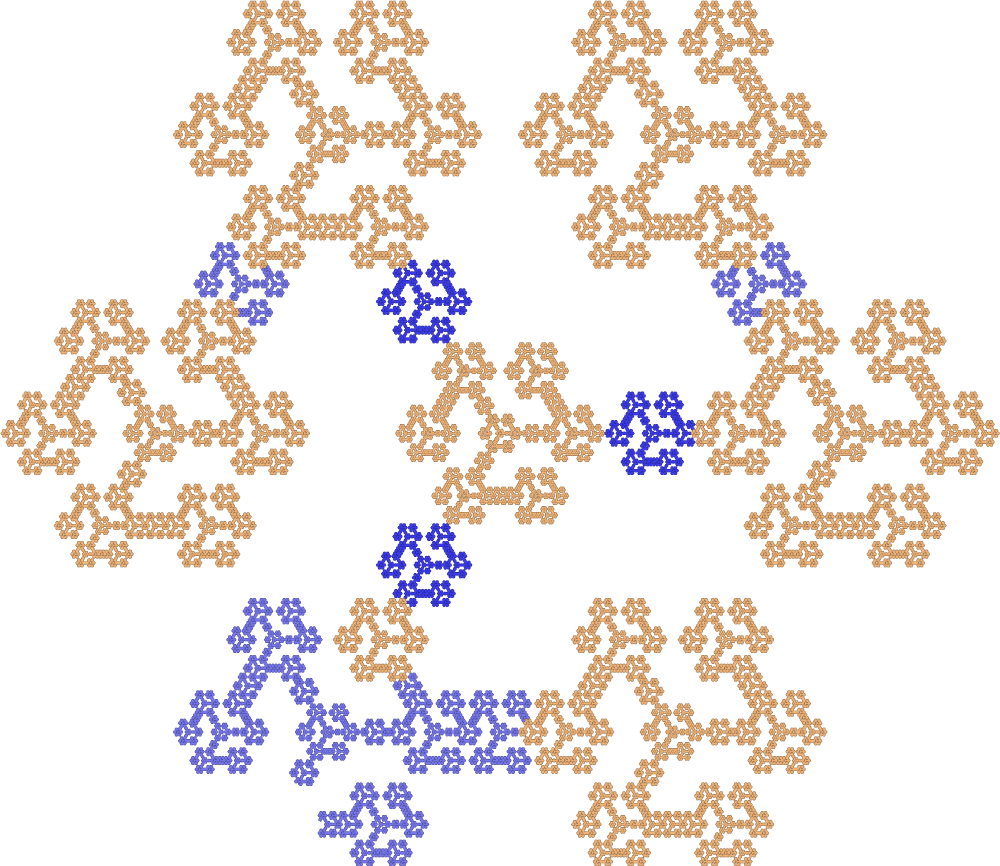
\includegraphics[width=0.35\textwidth]{EXTREME_5.3.png}
    \caption{Аттрактор граф-ориентированной системы для примера \ref{ex:5}}
    \label{fig:primer5}
\end{figure}

В очередной раз для вычисления размерности Хаусдорфа данного фрактала мы  представили его как компоненту аттрактора граф-ори\-ен\-ти\-ро\-ван\-ной системы (см. Рисунок \ref{fig:primer5} из Приложения 5) и вычислили размерность подобия этой системы:

$$
\begin{cases}
6a^s+3xa^{2s}+3ya^{2s}+(1-2a-2a^2+2a^4)^s=1\\
4a^s+3xa^{2s}+3ya^{2s}+3ya^{2s}+(1-2a-2a^2+2a^4)^s=x\\
5a^s+a^{2s}+3xa^{2s}+3ya^{2s}+xa^s+(1-2a-2a^2+2a^4)^s=y
\end{cases}
$$
Отсюда размерность граф-ориентированной системы есть $s\approx1.684053$.
\end{example}

\newpage
\section*{Заключение}
\addcontentsline{toc}{section}{Заключение}
Для нашего исследования мы построили пять самоподобных множеств с перекрытиями по подкопиям меньшего порядка. 
Для каждого из примеров была вычислена размерность подобия. Поскольку перекрытия при вычислении размерности данным способом учитывались несколько раз, размерность Хаусдорфа данных фракталов будет меньше вычисленной размерности подобия.

Чтобы вычислить искомую размерность Хаусдорфа, мы представили каждый фрактал с перекрытием в виде компоненты аттрактора граф-ориентированной системы без перекрытий.
Размерность подобия этой граф-ориентированной системы будет равна размерности Хаусдорфа изначального фрактала с перекрытиями.

Все самоподобные множества были построены в {\em IFStile}  и их изображения добавлены в текст проекта. Аттракторы граф-ориентированных системы также были построены, а изображения добавлены в приложения.

Стоит отметить важную закономерность. 
Во всех примерах, кроме примера \ref{ex:4}, использовались пересечения по подкопиям довольно маленького размера, и размерность падала на небольшие значения (на нес\-коль\-ко сотых).
В примере \ref{ex:4} были пересечения по подкопиям значительного размера, и размерность просела значительно (на $\approx0.23$).
Значит чем значительнее перекрытие, тем сильнее проседает размерность Хаусдорфа относительно размерности подобия.


\newpage
\addcontentsline{toc}{section}{Список литературы} % Добавляем раздел в содержание
\begin{thebibliography}{9}
\bibitem{bib:1}
    \textbf{Kenneth Falconer},
    Fractal Geometry: Mathematical Foundations and Applications,
    John Wiley $\&$ Sons, Ltd, 2014, 400 p.

\bibitem{bib:2}
    \textbf{Christoph Bandt and Siegfried Graf},
    Self-similar sets 7. A characterization of self-similar fractals with positive Hausdorff measure,
    Proceedings of the A.M.S., Vol. 114, N. 4 (1992), p. 995--1001

\bibitem{bib:3}
    \textbf{Сергей Деменюк},
    Просто фрактал,  
    ООО <<Страта>> (2012), 168 с.\end{thebibliography}


\newpage
\section*{Приложения}
\addcontentsline{toc}{section}{Приложения}

\lstset
    { %
    % language=aifs, % выбор языка для подсветки
    % inputencoding=utf8, % для кириллицы
    % extendedchars=\true, % использование не-ASCII символов
    % keepspaces=true, % Пробелы между словами в кириллице 
    basicstyle=\small\tt, % размер и начертание шрифта для подсветки кода
    numbers=left, % где поставить нумерацию строк (слева\справа)
    numberstyle=\small, % размер шрифта для номеров строк
    stepnumber=1, % размер шага между двумя номерами строк
    numbersep=15pt, % как далеко отстоят номера строк от подсвечиваемого кода
    % backgroundcolor=\color{white}, % цвет фона подсветки
    showspaces=false, % показывать или нет пробелы специальными отступами
    showstringspaces=false, % показывать или нет пробелы в строках
    showtabs=false, % показывать или нет табуляцию в строках
    % frame=single, % рисовать рамку вокруг кода
    tabsize=4, % размер табуляции по умолчанию равен 4 пробелам
    captionpos=t, % позиция заголовка вверху [t] или внизу [b] 
    breaklines=true, % автоматически переносить строки (да\нет)
    breakatwhitespace=true, % переносить строки только если есть пробел
    escapeinside={\%*}{*)}, % если нужно добавить комментарии в коде
    morecomment=[l][\color{gray}]{\#}, % символ комментария и цвет
    literate=  % костыль для отображения и закраски кириллицы (только utf8)
        {а}{{\selectfont\char224}}1 
        {б}{{\selectfont\char225}}1
        {в}{{\selectfont\char226}}1
        {г}{{\selectfont\char227}}1
        {д}{{\selectfont\char228}}1
        {е}{{\selectfont\char229}}1
        {ё}{{\"e}}1
        {ж}{{\selectfont\char230}}1
        {з}{{\selectfont\char231}}1
        {и}{{\selectfont\char232}}1
        {й}{{\selectfont\char233}}1
        {к}{{\selectfont\char234}}1
        {л}{{\selectfont\char235}}1
        {м}{{\selectfont\char236}}1
        {н}{{\selectfont\char237}}1
        {о}{{\selectfont\char238}}1
        {п}{{\selectfont\char239}}1
        {р}{{\selectfont\char240}}1
        {с}{{\selectfont\char241}}1
        {т}{{\selectfont\char242}}1
        {у}{{\selectfont\char243}}1
        {ф}{{\selectfont\char244}}1
        {х}{{\selectfont\char245}}1
        {ц}{{\selectfont\char246}}1
        {ч}{{\selectfont\char247}}1
        {ш}{{\selectfont\char248}}1
        {щ}{{\selectfont\char249}}1
        {ъ}{{\selectfont\char250}}1
        {ы}{{\selectfont\char251}}1
        {ь}{{\selectfont\char252}}1
        {э}{{\selectfont\char253}}1
        {ю}{{\selectfont\char254}}1
        {я}{{\selectfont\char255}}1
        {А}{{\selectfont\char192}}1
        {Б}{{\selectfont\char193}}1
        {В}{{\selectfont\char194}}1
        {Г}{{\selectfont\char195}}1
        {Д}{{\selectfont\char196}}1
        {Е}{{\selectfont\char197}}1
        {Ё}{{\"E}}1
        {Ж}{{\selectfont\char198}}1
        {З}{{\selectfont\char199}}1
        {И}{{\selectfont\char200}}1
        {Й}{{\selectfont\char201}}1
        {К}{{\selectfont\char202}}1
        {Л}{{\selectfont\char203}}1
        {М}{{\selectfont\char204}}1
        {Н}{{\selectfont\char205}}1
        {О}{{\selectfont\char206}}1
        {П}{{\selectfont\char207}}1
        {Р}{{\selectfont\char208}}1
        {С}{{\selectfont\char209}}1
        {Т}{{\selectfont\char210}}1
        {У}{{\selectfont\char211}}1
        {Ф}{{\selectfont\char212}}1
        {Х}{{\selectfont\char213}}1
        {Ц}{{\selectfont\char214}}1
        {Ч}{{\selectfont\char215}}1
        {Ш}{{\selectfont\char216}}1
        {Щ}{{\selectfont\char217}}1
        {Ъ}{{\selectfont\char218}}1
        {Ы}{{\selectfont\char219}}1
        {Ь}{{\selectfont\char220}}1
        {Э}{{\selectfont\char221}}1
        {Ю}{{\selectfont\char222}}1
        {Я}{{\selectfont\char223}}1
    }


\begin{lstlisting}[name=aifs,label=list:prev,caption=Описание команд и родительского блока]
@sim  # 
$a=h  # блок скрыт
kx1=0
ky1=0
kx2=1
ky2=1
ret=[kx1,ky1]*[(kx2-kx1),(ky1-ky2),(ky2-ky1),(kx2-kx1)]

@rot  # команда "поворот"
$a=h  # блок скрыт
ka=0
ret=[cos(ka),-sin(ka),sin(ka),cos(ka)]

@G
$a=h  # блок скрыт
$n=zagot  # имя блока
$dim=2  # размерность
pi=2*asin(1)
&A=(0.5|[0.5,0]*0.5)*A  # единичный отрезок
&Ar=(1|[0.8,0]*rot(2*pi/3)*0.05)*A  # стрелка
&P0=(1|rot(pi/2)|[0,1]|[1,0]*rot(pi/2))*A
\end{lstlisting}


\begin{lstlisting}[name=aifs,label=list:prev,caption=Код примера \ref{ex:1}]
@G4:G
$a=c  # блок не скрыт
$n=den_kv_3_2  # имя блока
q=(sqrt(3)-1)/2  # 3*p-2*p^3=1
s1=q
s2=[0.5-0.5*q,0.5-0.5*q]*q
s3=[1-q,1-q]*q
s4=[0.5+0.5*q,0]*(3-3^.5)/4
s5=[0,0.5+0.5*q]*(3-3^.5)/4
S=s1|s2|s3|s4|s5
K=S*K
P1=(1|S)*P0
Z1=P1|K
K1=(s1|s3|s4|s5)*K1|s2*K2
K2=(s4|s5|s3*(s1|s4|s5)|s1*(s3|s4|s5))*K1|(s1|s3|1)*s2*K2
\end{lstlisting}


\begin{lstlisting}[name=aifs,label=list:prev,caption=Код примера \ref{ex:2}]
@G1:G
$a=c  # блок не скрыт
$n=den_kv_1_1  # имя блока
q=0.4406197005381991
s1=q
s2=[1-q,0]*q
s3=[0,1-q]*q
s4=[1-q,1-q]*q
s5=[0.5-q*q/2,0.5-q*q/2]*q^2
S=s1|s2|s3|s4|s5
K=S*K
K1=s1*K1|s2*K1|s3*K1|s4*K1|s5*K2
K2=s5*K2|s1*s5*K2|s2*s5*K2|s3*s5*K2|s4*s5*K2|
    s2*s1*K1|s3*s1*K1|s4*s1*K1|
    s1*s2*K1|s3*s2*K1|s4*s2*K1|
    s1*s3*K1|s2*s3*K1|s4*s3*K1|
    s1*s4*K1|s2*s4*K1|s3*s4*K1
P1=(1|S)*P0
Z1=P1|K
\end{lstlisting}


\begin{lstlisting}[name=aifs,label=list:prev,caption=Код примера \ref{ex:3}]
@G7
$dim=2
$n=den_tr
$a=h
pi=2*asin(1)
&A=(0.5|[0.5,0]*0.5)*A
p=$number($real(0.3,0.4))
r3=[1,0]*rot(2*pi/3)
P0=(1|r3|r3^2)*A
s1=p
s2=r3*p
s3=r3^2*p
s4=[p-p^3,0]*p^2
s5=r3*s4
s6=r3^2*s4
x1=p+p^2/2-p^3
y1=3^.5*p^2/2
x2=1-p/2-p^2+p^3/2
y2=(p-p^3)*3^.5/2
s7=sim(x1,y1,x2,y2)
dd=((x2-x1)^2+(y2-y1)^2)^0.5
S=s1|s2|s3|s4|s5|s6|s7
P1=(1|S)*P0
K=S*K
K1=(s1|s2|s3|s7)*K1|(s4|s5|s6)*K2
K2=(s2|s3|s7)*K1|(s4|s5|s6)*K2

@:G7
$n=den_tr
p=.394930843634698 #Lip(s7)=0.3072016617022929
\end{lstlisting}


\begin{lstlisting}[name=aifs,label=list:prev,caption=Код примера \ref{ex:4}]
@G1
$dim=2 # размерность
$n=name # имя блока
pi=2*asin(1)
A=(0.5|[0.5,0]*0.5)*A
P0=(1|rot(pi/2)|[0,1]|[1,0]*rot(pi/2))*A
Tr=(1|rot(pi/3)|[1,0]*rot(2*pi/3))*A
Ro=0.5*(rot(-pi/3)|[1,0]*rot(-2*pi/3)|
    rot(pi/3)|[1,0]*rot(2*pi/3))*A
Tp=(1|rot(pi/3)*0.5|[1,0]*rot(2*pi/3)*0.5|
    [0.25,3^0.5/4]*0.5)*A
T2=(1|[0.5,0]|[0.25,0]|[0.25,3^0.5/4])*0.5*T2
K1=(0.5*K1|[0.5,0]*0.5*K1|[0.25,3^0.5/4]*0.5*K1)|
    ([3/8,3^0.5/8]*0.5*K2)
K2=(0.5*K1)|([0.125,-(3^0.5)/8]*0.5*K2)
KK1=((1|[0.5,0]|[0.25,3^0.5/4])*0.5*Tr)|
    ([3/8,3^0.5/8]*0.5*Ro)
KK2=Ro|0.5*Tr|[0.125,-(3^0.5)/8]*0.5*Ro
r=[1,0]*rot(2*pi/3)
ZZ1=Tr|[0.25,0]*0.5*Tr|[0.25,3^0.5/4]*0.5*Tr|
    [0.25,3^0.5/4]*rot(4*pi/3)*0.5*Tp|[1,0]*rot(2*pi/3)*0.5*Tp
ZZ2=Tp|[0.5,0]*0.5*Tp|[3/8,3^0.5/8]*0.5*Tp|0.5*r*Tr
ZZ3=Tp|0.5*Tp|[0.125,3^0.5/8]*0.5*Tp|[0.5,0]*0.5*r*r*Tr
Z1=[0.25,0]*0.5*Z1|[0.25,3^0.5/4]*0.5*Z1|
    [0.25,3^0.5/4]*rot(4*pi/3)*0.5*Z2|[1,0]*rot(2*pi/3)*0.5*Z3
Z2=[0.5,0]*0.5*Z2|[3/8,3^0.5/8]*0.5*Z2|0.5*r*Z1
Z3=0.5*Z3|[0.125,3^0.5/8]*0.5*Z3|[0.5,0]*0.5*r*r*Z1
\end{lstlisting}


\begin{lstlisting}[name=aifs,label=list:prev,caption=Код примера \ref{ex:5}]
@G6
$dim=2
$n=den six 3.2 4.3 
pi=2*asin(1)
r6=[1,0]*rot(pi/3)
&I=(0.5|[0.5,0]*0.5)*I  # отрезок
P0=(1|r6|r6^2|r6^3|r6^4|r6^5)*I # шестиугольник
a=(5^0.5-1)/4
s1=a
s2=r6*a*r6^-1
s3=r6^2*a*r6^-2
s4=r6^3*a*r6^-3
s5=r6^4*a*r6^-4
s6=r6^5*a*r6^-5
s7=[1.5*a-2*a^3+0.5*a^2,(a-a^2)*3^0.5/2]*a^2
s8=r6^2*s7
s9=r6^4*s7
s10=[a-a^4,(a-a^4)*3^0.5]*a^2
s11=r6^2*s10
s12=r6^4*s10
s13=[a+a^2-a^4,(a+a^2-a^4)*3^0.5]*(1-2*a-2*a^2+2*a^4)
S=s1|s2|s3|s4|s5|s6|s7|s8|s9|s10|s11|s12|s13
P1=(1|S)*P0
K=S*K
K1= (s1|s2|s3|s4|s5|s6|s13)*K1|
    (s7|s8|s9)*K2|
	(s10|s11|s12)*K3
K2= (s1|s2|s4|s5|s13)*K1|
    (s7|s8|s9)*K2|
	(s10|s11|s12)*K3
K3= (s2|s3|s4|s5|s6|s13|s1*s4)*K1|
    (s7|s8|s9|s1*r6^4)*K2|
	(s10|s11|s12)*K3
\end{lstlisting}


\end{document}
